\documentclass[12pt,a4paper,notitlepage]{report}
\usepackage[utf8]{inputenc}
\usepackage[czech]{babel}
\usepackage[pdftex]{graphicx} %pro vkládání obrázků v eps
\usepackage{hyperref} %pro kliknutelné linky
\usepackage[small,bf,belowskip=0.2cm]{caption} %změna stylu popisku a mezery před a za
\usepackage{sectsty} % pro jednoduché přestylování nadpisů
\usepackage{booktabs} % kvuli siunitx v tabulkach
\usepackage{array} %siunitx a centrovani tabulek
\usepackage{enumitem} %pro umravnění mezer v enumerate + změnu popisků
\usepackage{subfig}


%pro zdrojaky
\usepackage{listingsutf8}
\lstset{language=C,basicstyle=\footnotesize,numbers=left,showspaces=false,showstringspaces=false,numberstyle=\footnotesize,frame=single,title=\lstname,breaklines=true,inputencoding=utf8/latin2
} 

\usepackage[round]{natbib}
\usepackage{tabularx}
\usepackage{siunitx} %pro sazbu fyzikálních jednotek
\usepackage[top=2.5cm, bottom=2.5cm, left=2.5cm, right=2cm]{geometry} %nastaveni okraju a vzdalenosti cislovani

%pro vertikalni mezery u nadpisu
\usepackage[compact]{titlesec}
\titlespacing{\section}{0pt}{*3}{*0} %před a za
\titlespacing{\subsection}{0pt}{*3}{*0}
%\titlespacing{\subsubsection}{0pt}{*1}{*0}

\setlength{\textfloatsep}{0cm} %mezera za tabulkami


%nastaveni zobrazovani cisel jak je u nas zvykem :)
\sisetup{output-decimal-marker={,},exponent-product = \cdot, list-final-separator = { a }  }

%vypne vypisovani Kapitola u \chapter
\makeatletter
\def\@makechapterhead#1{%
  \vspace*{\p@}%
  {\parindent \z@ \raggedright \normalfont
    \interlinepenalty\@M
     \fontsize{17pt}{1}\selectfont \bfseries \thechapter\ \hspace{10pt} #1\par\nobreak
    \vskip 10\p@
  }}
\makeatother{}

%aby stejne vypadala i chapter*
\makeatletter
\def\@makeschapterhead#1{%
  \vspace*{\p@}%
  {\parindent \z@ \raggedright \normalfont
    \interlinepenalty\@M
     \fontsize{17pt}{1}\selectfont \bfseries #1\par\nobreak
    \vskip 10\p@
  }}
\makeatother{}

%chapter ted nedelani \newpage + pridana vspace
\makeatletter
\renewcommand\chapter{\vspace{0.7cm}\par%
  \thispagestyle{plain}%
  \global\@topnum\z@
  \@afterindentfalse
  \secdef\@chapter\@schapter}
\makeatother
{}

%velikost nadpisu
\sectionfont{\vspace{2mm}\fontsize{14pt}{1}\selectfont}
\subsectionfont{\vspace{2mm}\fontsize{12pt}{1}\selectfont}

%vlastni prikazy
\newcommand{\flu}{Ansys Fluent}

\addtocontents{toc}{\protect\thispagestyle{empty}} %odstraní číslování na stránce obsahu
\setcounter{tocdepth}{1}

\begin{document}
    \abovedisplayshortskip=-12pt %vertikální mezera před rovnicí
    %\belowdisplayshortskip=8pt  %vertikální mezera za rovnicí
    
    \abovedisplayskip=-10pt %vertikální mezera před rovnicí \noindent
    %\belowdisplayskip=0pt
	
	\pagestyle{empty} 
	\selectlanguage{czech}
	\begin{center}
{\Large VYSOKÁ ŠKOLA CHEMICKO-TECHNOLOGICKÁ V PRAZE\\}
{\large Fakulta chemicko-inženýrská\\
\textbf{Ústav chemického inženýrství}\\}
\vspace{15mm}

\begin{figure}[!h]
\begin{center}

\includegraphics[angle=0,width=27mm]{images/logo_vscht.eps}
\end{center}
\end{figure}

\vspace{25mm}

{\huge \textbf{DIPLOMOVÁ PRÁCE\\}}
\vspace{10mm}
{\large \textbf{VÝPOČET VZNOSU PEVNÉ ZRNITÉ FÁZE V~MECHANICKY MÍCHANÉ NÁDOBĚ METODOU CFD\\}}
\end{center}
\vspace{25mm}

\begin{tabular}{p{50mm}lp{50mm}}
Vypracoval: & \textbf{Bc.\,Tomáš Antecký}\\
\\
Vedoucí práce: & Doc.\,Dr.\,Ing.\,Milan Jahoda \\

\\
Studijní program: & Procesní inženýrství a informatika \\
\\
Studijní obor: & Chemické inženýrství, bioinženýrství  \\
	& a matematické modelování procesů\\
\end{tabular}

  \section*{Souhrn}

	\tableofcontents{}
	\pagestyle{plain}
  \newpage
  \setlength{\baselineskip}{1.5\baselineskip}
	\setcounter{page}{1}
	
  \chapter{Úvod}


  \chapter{Teoretická část}

\section{Počítačová dynamika tekutin}

\section{Vícefázové modely}
V současnosti existuje řada matematických modelů, které popisují vícefázové proudění. Následující kapitola obsahuje přehled modelů, které jsou vhodné k simulaci suspendace v mechanicky míchaných nádobách.

\subsection{Eulerian-Lagrangian}
Tento typ modelu uvažuje primární tekutou fází jako kontinuum s dispergovanou sekundární fází. Pro primární fázi je řešena rovnice kontinuity spolu s Navierovými-Stokesovými rovnicemi, zatímco pro dispergovanou fázi je řešena trajektorie každé částice separátně. Jednotlivé fáze si mohou mezi sebou vyměňovat hmotu, hybnost a energii, avšak vzájemné interakce částic nebo jejich rozpad jsou zanedbány. Model Eulerian-Lagrangian je především vhodný pro systémy, kde objemový zlomek dispergované fáze nepřesáhne \SI{10}{\percent} např: rozprašovací sušárny, cyklóny nebo spalování uhlí či kapalného paliva. 

Řešením bilance sil působící na částici (rov. \ref{eq:dpm}) je získána její trajektorie v daném časovém okamžiku.

\begin{equation}
	\frac{d\vec{v}_{p}}{dt} = \vec{F}_{D}(\vec{v}_{f} - \vec{v}_{p}) + \frac{\vec{g}(\rho_{p} - \rho_{f})}{\rho_{p}} + \frac{\vec{F}_{ad}}{\rho_{p}}
	\label{eq:dpm}
\end{equation} 

\noindent Kde jednotlivé členy značí:

\begin{itemize}[itemsep=0pt,parsep=0pt,partopsep=0pt,topsep=0pt]
  \item $\vec{v}_{p}$ vektor rychlosti dané částice
  \item $\vec{v}_{f}$ vektor rychlosti tekutiny
  \item $\rho_{p}$, $\rho_{f}$ hustotu částice resp. tekutiny
  \item $\vec{g}$ gravitační zrychlení
  \item $\vec{F}_{D}$ odporová síla
  \item $\vec{F}_{ad}$ další síly (např: tlaková, zdánlivá síla, síla zahrnující vliv rotace atd.)
\end{itemize}

\subsection{Eulerian-Eulerian}
U modelu Eulerian-Eulerian jsou jednotlivé fáze považovány za prostupující se kontinua a každý bod v systému obsahuje informaci o objemovém zlomku dané fáze. Z tohoto popisu je zřejmé, že suma objemových zlomků přes všechny fáze v libovolném bodě se vždy musí rovnat jedné. 

\begin{equation}
	\sum_{i=1}^n \alpha_{i} = 1
	\label{eq:volfrac}
\end{equation} 

\noindent Jednotlivé fáze mohou být kapalné, plynné nebo pevné a jejich celkový počet není teoreticky limitován. Pro každou fázi se řeší rovnice kontinuity (\ref{eq:conti}) a sada rovnic pro hybnost. (\ref{eq:moml}). K výměně hybnosti mezi jednotlivými fázemi slouží mezifázové členy v těchto rovnicích. Pokud dochází k přenosu tepla nebo hmoty je třeba tuto skutečnost zohlednit v bilanci energie a hmoty.    

Když probíhá výměna hmoty mezi jednotnými fázemi tak rovnice kontinuity pro $i$-tou fázi má tvar:

\begin{equation}
	\frac{\partial}{\partial t} (\alpha_{i}\rho_{i}) +  \nabla \cdot (\alpha_{i}\rho_{i}\vec{v}_{i}) = 0
	\label{eq:conti}
\end{equation}

\noindent Rovnice hybnosti pro $i$-tou fázi za stejných předpokladů lze zapsat jako:

\begin{equation}
	\frac{\partial}{\partial t} (\alpha_{i}\rho_{i}\vec{v}_{i}) + \nabla \cdot (\alpha_{i}\rho_{i} \vec{v}_{i} \otimes \vec{v}_{i}) = -\alpha_{i} \nabla p + \nabla \cdot \bar{\tau}_{i} + \alpha_{i}\rho_{i}\vec{g} + \sum_{j=1}^n \vec{R}_{ji} + \vec{F}_{ext} + \vec{F}_{int}
	\label{eq:moml}
\end{equation}

\noindent kde $p$ je tlak, $\bar{\tau}_{i}$ je deviátor tenzoru napětí, jehož konkretní tvar závisí na typu uvažované fáze, a $\alpha_{i}\rho_{i}\vec{g}$ má význam gravitační síly působící na objemový element. Člen $\vec{R}_{ji}$ představuje mezifázovou odporovou sílu mezi $i$-tou a $j$-tou fází, $\vec{F}_{ext}$ má význam dalších objemových sil a $\vec{F}_{int}$ zahrnuje povrchové síly působící na $i$-tou fázi vlivem ostatních fází. 

\subsection{Eulerian-Granular}
Model Eulerian-Granular se liší od předchozího tím, že  popis chování pevné fáze byl odvozen s využitím kinetické teorie, která je například známá ze statistického popisu plynů. U tohoto modelu se viskozita pevné fáze mění v závislosti na interakcích s ostatními částice a primární fází. Na rozdíl od modelu Eulerian-Eulerian model Eulerian-Granular umožňuje nastavit maximální hodnotu objemového zlomku pevné fáze, která je pro sférické částice typicky kolem hodnoty \num{0.6}. Mezi nejčastější aplikace patří simulace fluidních loží nebo suspendace v mechanicky míchaných nádobách.

Bilanci hybnosti pro pevnou fázi $s$ má tvar:

\begin{equation}
	\frac{\partial}{\partial t} (\alpha_{s}\rho_{s}\vec{v}_{s}) + \nabla \cdot (\alpha_{s}\rho_{s} \vec{v}_{s} \otimes \vec{v}_{s}) = -\alpha_{s} \nabla p - \nabla p_{s} + \nabla \cdot \bar{\tau}_{s} + \alpha_{s}\rho_{s}\vec{g} + \sum_{j=1}^n \vec{R}_{ji} + \vec{F}_{ext} + \vec{F}_{int}
	\label{eq:momls}
\end{equation}
  
\noindent Člen $p_{s}$ je tlak pevné fáze, který je důsledkem neelastických srážek mezi částicemi, a $\bar{\tau}_{s}$ je deviátor tenzoru napětí pro pevnou fázi.       

\section{Mezifázová odporová síla}

Člen mezifázové odporové síly $\vec{R}_{ji}$ v rovnici \ref{eq:moml} nebo \ref{eq:momls} nejvýznamněji přispívá do popisu interakce mezi jednotlivými fázemi, a proto správnost popisu tohoto členu zásadně ovlivňuje kvalitu výsledné simulace. 

Tuto sílu lze rozepsat jakou součin koeficientu mezifázového sdílení hybnosti a relativní rychlosti $i$-té a $j$-té fáze.

\begin{equation}
	\sum_{j=1}^n \vec{R}_{ji} = K_{ji} \left( \vec{v}_{j} - \vec{v}_{i} \right)
	\label{eq:kij}
\end{equation}

\noindent Z definice \ref{eq:kij} je jasné, že platí vztahy $\vec{R}_{ji} = -\vec{R}_{ij}$ a $\vec{R}_{ii} = 0$. Vzorec pro výpočet $K_{ji}$ se obecně liší podle toho jaké typy fází spolu interagují. Pokud se jedná o interakci kapalina-pevná fáze, tak koeficient mezifázového sdílení hybnosti má tvar:

\begin{equation}
	K_{fs}= \frac{3\alpha_{s}C_{D}\rho_{f}|\vec{v}_{s} - \vec{v}_{f}|}{4d_{s}}
	\label{eq:kfs}
\end{equation}
  
\noindent Symbol $d_{s}$ značí průměr pevných částic a $C_{D}$ koeficient odpor, kterým se právě ovlivňuje chování odporové síly. Tento koeficient může být obecně složitou funkcí relativní rychlosti pohybu částice, její velikosti, hustotou a viskozitou tekutiny případně dalších veličin.   

V současnosti existuje řada modelů pro koeficient odporů, které se liší podle toho, pro jaký účel byly navrženy. Jedním z nejznámějších je model, který navrhli \citet{schi32}. Autoři získali vztah \ref{eq:schlneu} pro výpočet koeficientu odporu na základě experimentálního měření rychlosti usazování sférické částice ve stagnantním sloupci kapaliny.    
 
\begin{equation}
	\label{eq:schlneu}
  C_{D0} = \left\{ \begin{array}{ll}
  \frac{24}{Re_{p}}  \left( 1 + \num{0.15}Re_{p}^{\num{0.687}} \right) & Re_{p} \le 1000\\
  \num{0.44} & Re_{p} > 1000\\
  \end{array} \right.
\end{equation}

\noindent Ze vztahu \ref{eq:schlneu} je patrné, že Schillerova-Naumannova korelace je funkcí Reynoldsova kritéria pro částici, které je definováno jako:

\begin{equation}
	Re_{p}= \frac{\rho_{f}d_{s}|\vec{v}_{s} - \vec{v}_{f}|}{\eta_{f}}
	\label{eq:reyp}
\end{equation}

Bohužel odporový koeficient navržený Schillerem a Naumannem se ukázal jako nepříliš vhodný k popisu odporové síly v systémech s plně vyvinutým turbulentním prouděním. Proto řada autorů navrhl úpravu této korelace a některé z nich jsou uvedeny v tab. \ref{tab:cds}. Člen $\lambda$ se nazývá Kolmogorovo mikroměřítko je funkcí kinematické viskozity a disipace energie a určuje nejmenší velikost turbulentní vírů přítomných v systému. 

\begin{table}[h!]
\begin{center}
  

		\caption{Modely pro odporový koeficient v turbulentní oblasti proudění}
		\label{tab:cds}
\begin{tabular}{|c|c|>{\centering\arraybackslash}p{5cm}|}
  \hline
  
{\textbf{Autor}} & {\textbf{Koeficient odporu}} & {\textbf{Stanoveno na základě}} \\ \hline{}

\citet{pin01} & $C_{D} = C_{D0} \left( \num{0.4}\tanh\left(  \frac{16\lambda}{d_{s}} - 1  \right) \right) ^{-2}$ & měření rychlosti usazování v míchací nádobě \\ \hline
 
\citet{bru98} & $C_{D} = C_{D0} \left( 1 + \num{8.76e-4} \left( \frac{\lambda}{d_{s}} \right)^{3} \right)$ & experimentální studie Taylorova–Couetteova toku \\ \hline 

\citet{kho06} & $C_{D} = C_{D0} \left( 1 + \num{8.76e-5} \left( \frac{\lambda}{d_{s}} \right)^{3} \right)$ & úpravy Brucatova vztahu pro míchací nádoby  \\ \hline 

\end{tabular}
\end{center}
\end{table}









  \chapter{Experimentální část}
Experimentální studii suspendace v~mechanicky míchané nádobě provedla \citet{pav11} v~rámci své bakalářské práce na Ústavu chemického inženýrství VŠCHT Praha.

\section{Popis experimentu}
\label{chap:exp}
Náplní experimentu bylo měření průběhu suspendace v~systému kapalina-pevná fáze spolu se stanovením doby homogenizace. K~provedení experimentu byla využita válcová nádoba z~plexiskla o~vnitřním průměru $T=\SI{0.29}{\meter}$ s~plochým dnem, jenž byla opatřena čtyřmi radiálními narážkami o~šířce $b=T/10$. Výška plnění nádoby byla zvolena $H=T$. Do nádoby $C=T/3$ ode dna bylo umístěno šestilopatkové míchadlo se šikmo skloněnými lopatkami (úhel zkosení \SI{45}{\degree}) a celkovým průměrem  $D=T/3$. 
\begin{figure}[h!]
\centering
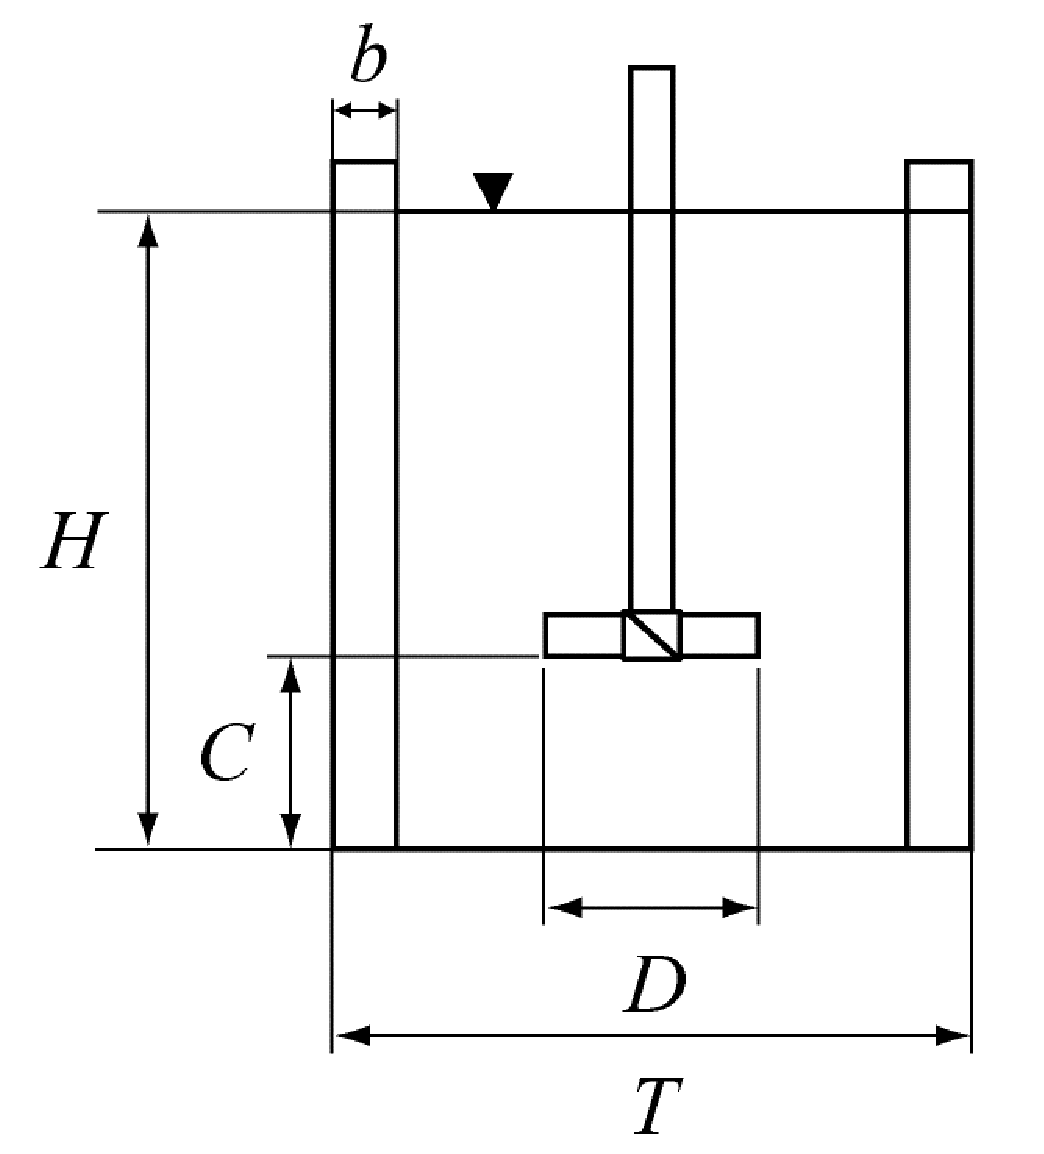
\includegraphics[scale=0.44]{images/mujedit.eps}
\caption{Geometrie experimentu}
\label{fig:nadoba}
\end{figure} 
Detailnější geometrie použitého míchadla je rozkreslena na obr. \ref{fig:imp}. Směr rotace hřídele byl volen tak, aby míchadlo vytvářelo proudění proti dnu nádoby. Frekvence jeho otáčení se pohybovala v~intervalu od \SI{3}{\per\second} do \SI{9}{\per\second}, což přibližně odpovídá Reynoldsovu číslu pro míchání ($Re_{M}$) od \num{24500} do \num{73800}.
\begin{figure}[t]
\centering
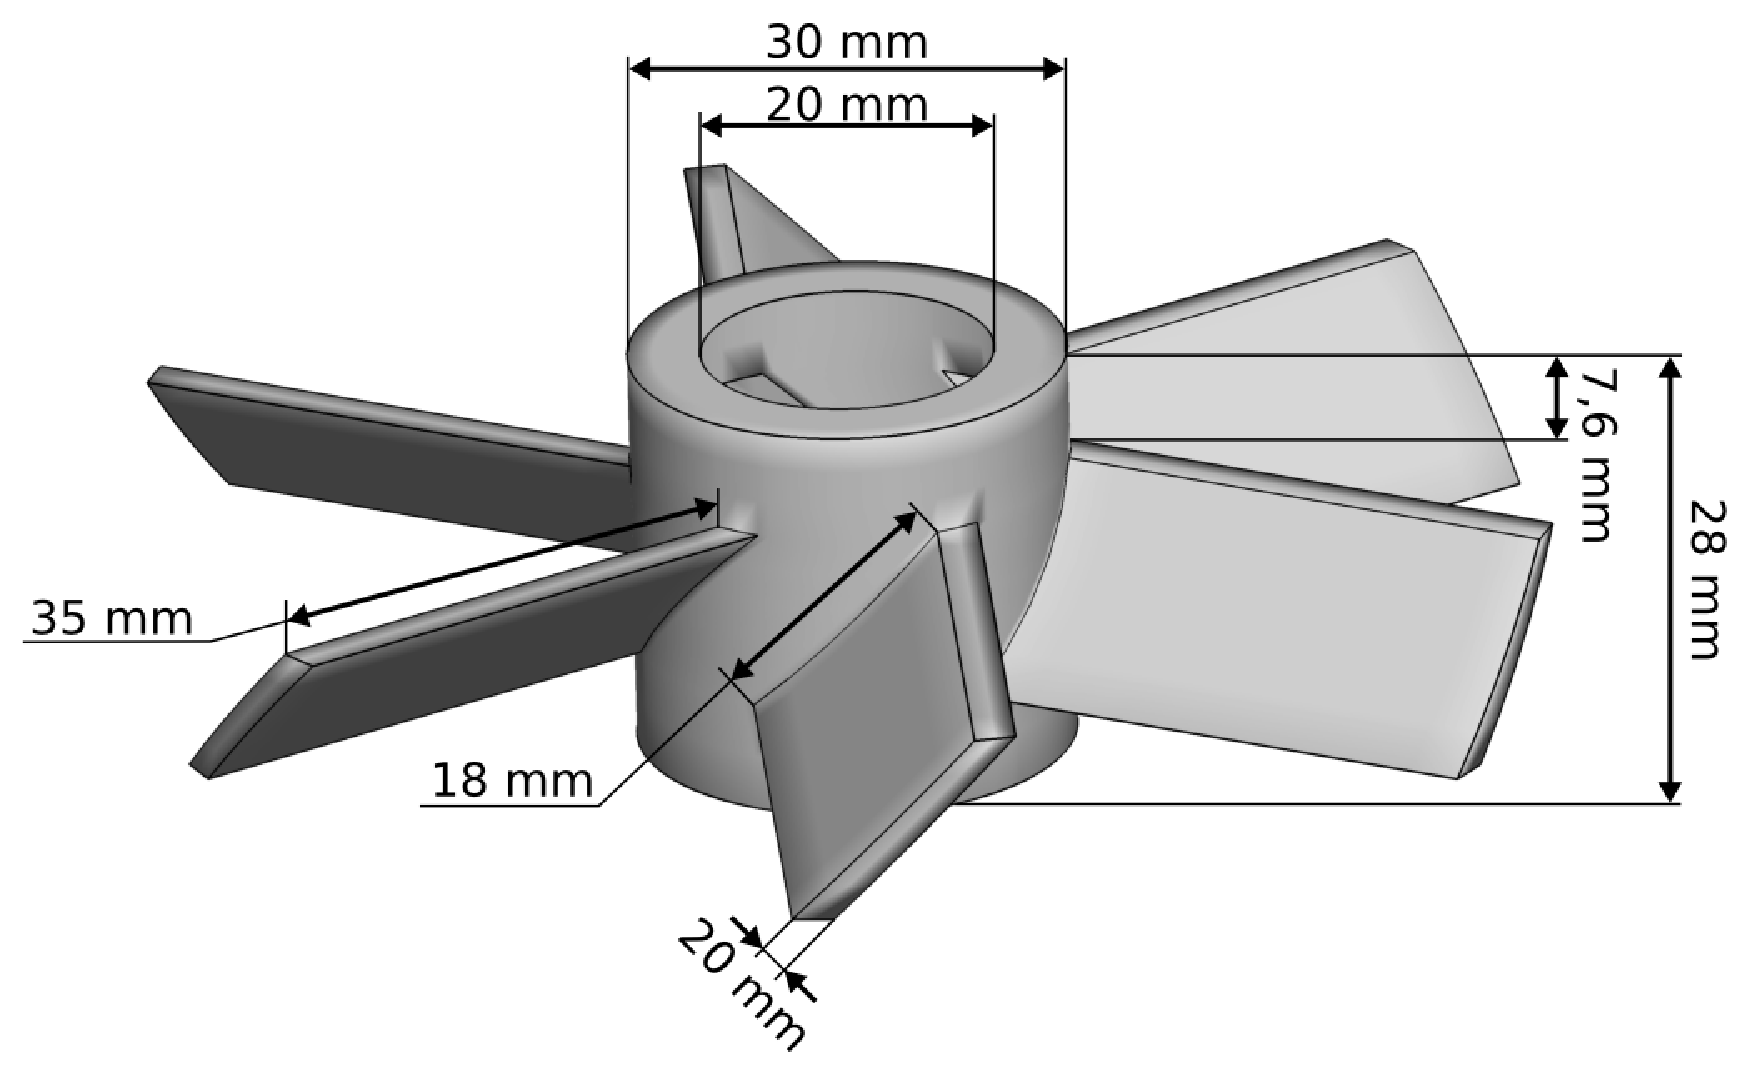
\includegraphics[scale=0.35]{images/imp.eps}
\caption{Geometrie míchadla}
\label{fig:imp}
\end{figure} 

Jako vsádka byla použita voda a polyvinylpyrrolidon (PVP), což je polymer rozpustný ve vodě s~newtonovských chováním. V~této práci byly využity dvě varianty této kapaliny \pvpP a \pvpS lišící se dynamickou viskozitou (\num{5} resp. \SI{7.5}{\milli\pascal\second}).  Pevnou fázi tvořily červené kuličky z~polyvinylchloridu (PVC) o~průměru \SI{1.02}{\milli\meter}. Vsádka postupně obsahovala 5, 10 a \volproc{15} těchto kuliček. Experimentálně stanovené vlastnosti kapalné a pevné fáze jsou shrnuty v~tab. \ref{tab:fyzvlast}. 
\begin{table}[h!]
\centering
\caption{Určené vlastnosti kapalné a pevné fáze}
\label{tab:fyzvlast}
\begin{tabular}{llrc}
\toprule
\textbf{Fáze} & \textbf{Veličina} & \textbf{Hodnota} &\textbf{Jednotka} \\
\midrule

voda \\
	& hustota & \num{999.50} & \si{\kilogram\per\cubic\meter} \\
	& dynamická viskozita & \num{1.138} & \si{\milli\pascal\second} \\
\pvpP \\
	& hustota & \num{1011.44} & \si{\kilogram\per\cubic\meter} \\
	& dynamická viskozita & \num{5.050} & \si{\milli\pascal\second} \\
\pvpS \\
	& hustota & \num{1024.18} & \si{\kilogram\per\cubic\meter} \\
	& dynamická viskozita & \num{7.615} & \si{\milli\pascal\second} \\
PVC \\
	& hustota & \num{1136.0} & \si{\kilogram\per\cubic\meter} \\
	& průměr & \num{1.02} & \si{\milli\meter} \\
	& mezerovitost & \num{0.384} & -- \\

\bottomrule
\end{tabular}
\end{table}

Pro stanovení průběhu homogenizace vsádky byla využita stopovací látka v~podobě chloridu sodného. Jeho roztok o~objemu přibližně \SI{5}{\milli\litre} byl nastříknut na volnou hladinu mezi narážku a hřídel míchadla. Koncentrace této látky byla měřena pomocí vodivostní sondy umístěné na opačné straně nádrže ve výšce $w = T/4$ ode dna. Výstupní analogový signál z~čidla o~vzorkovací frekvenci \SI{3}{\hertz} byl po zpracování A/D převodníkem uložen v~připojeném počítači k~dalšímu zpracování. Zaznamenané hodnoty napětí byly následně přepočítány na bezrozměrnou koncentraci $c^{*}(t)$ podle vzorce:    
\begin{equation}
	c(t)^{*} = \frac{c(t) - c_{0}}{c_{\infty} - c_{0}} \approx \frac{U(t) - U_{0}}{U_{\infty} - U_{0}}
	\label{eq:bezkonU}
\end{equation}
přičemž symbol $U$ značí hodnotu napětí ve zvoleném čase a význam ostatních symbolů je stejný jako ve vztahu \ref{eq:bezkon}. Doba po které dosáhla fluktuace bezrozměrné koncentrace hodnoty menší než \SI{5}{\percent}, byla považována za dobu homogenizace ($t_{mix}$). 

Během experimentu byly také pořizovaly digitální fotografie míchaného systému lišící se koncentrací pevné fáze, použitou kapalnou vsádkou a rychlostí otáčení míchadla. Získané fotografie byly poté použity k~orientačnímu stanovení výšky vznosu pevné fáze. 

  
  \chapter{Výpočetní část}

\section{Tvorba geometrie}

Výpočetní doména byla vytvořena v programu Ansys DesignModeler podle geometrie uvedené v kapitole \ref{chap:exp}. Výsledná nestrukturovaná síť byla tvořena šestistěnnými a čtyřstěnnými buňkami o celkovém počtu \num{264398}. Průměrný objem buňky činil \SI{0.07}{\milli\litre} a průměrný skewness faktor \num{0.162}. Výpočetní doména je znázorněna na obr. \ref{fig:geo}, kde zelenou barvou je znázorněna rotační zóna kolem míchadla. 

\begin{figure}[h!]
\begin{center}
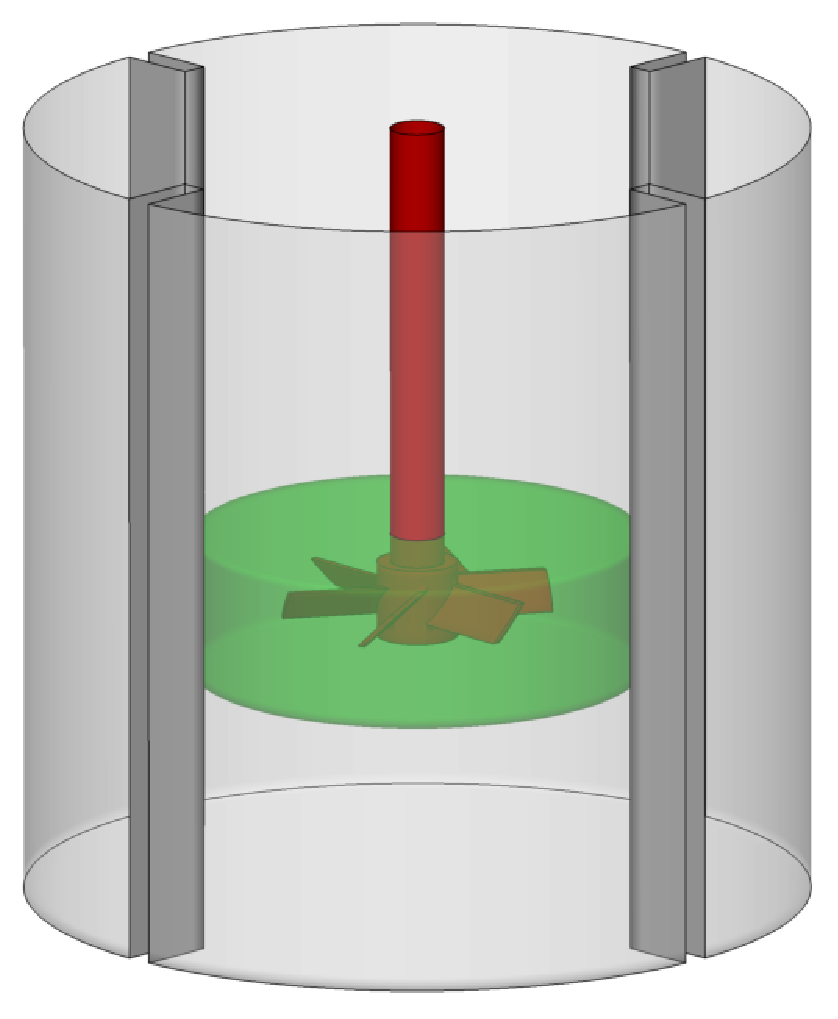
\includegraphics[scale=0.28]{images/geo.eps}
\caption{Výpočetní doména}
\label{fig:geo}
\end{center}
\end{figure} 

\section{Uživatelsky definové funkce}
Uživatelem definované funkce (UDF) jsou moduly načítané do softwaru \flu, jenž rozšiřují nebo upravují schopnosti řešiče. Například může se jednat o definovaní vlastních počátečních a okrajových podmínek, změnu materiálových vlastností a modifikaci simulačních modelů. Pro tvorbu zdrojových souborů se využívá programovací jazyk C, které jsou následně zkompilovaný do dynamické knihovny.

Všechny korelace pro odporový koeficient uvedené v tab. \ref{tab:cds} byly implementovány v podobě uživatelsky definovaných funkcí a jejich zdrojové kódy jsou uvedeny v kapitole Příloha.

\section{Vlastní CFD simulace}
K CFD simulaci byl využit komerční software \flu verze 12.1.4 do kterého byla načtena vytvořená výpočetní síť. Množství pevné fáze v míchací nádobě bylo zvoleno 5\,\%\,obj. pro všechny provedené výpočty. Pohyb míchadla byl simulován pomocí metody rotující sítě (sliding mesh) a jeho rychlost otáčení byla zvolena \SI{7}{\per\second}. Pro popis turbulentního proudění byl
využit standardní $k\mbox{-}\epsilon$ model s disperzní modifikací pro vícefázové proudění. Časový krok nestacionární simulace byl zvolen \num{0.001} sekundy. Postupně byly využity všechny korelace pro odporový koeficient uvedeny v tab. \ref{tab:cds} spolu s klasickým Schillerovým-Naumannovým vztahem. Simulace probíhala na počítači HP Z600 osazený dvěma procesory Intel Xeon X5570 a pamětí 24 GB s operačním systémem CentOS 5.3 x86-64. Doba výpočtu jedné reálné vteřiny trvala přibližně XX hodin.



  \chapter{Výsledková část}
Následující kapitola shrnuje získané výsledky pomocí CFD simulace popsané v předcházejících odstavcích. 

Na obr. \ref{fig:vecfield} je znázorněno vektorové pole rychlosti kapaliny v řezu nádobou a čase \SI{6}{\second}, což již lze považovat za poměrně ustálený stav. Z obrázku je dobře patrný vznikl sekundárních cirkulačních smyček v prostoru pod míchadlem. Tento jev byl experimentálně pozorován řadou autorů (např. \citet{hos10}) při zvolené světlé výšce míchadla od $C=T/2$ do $C=T/6$.  

\begin{figure}[h!]
\begin{center}
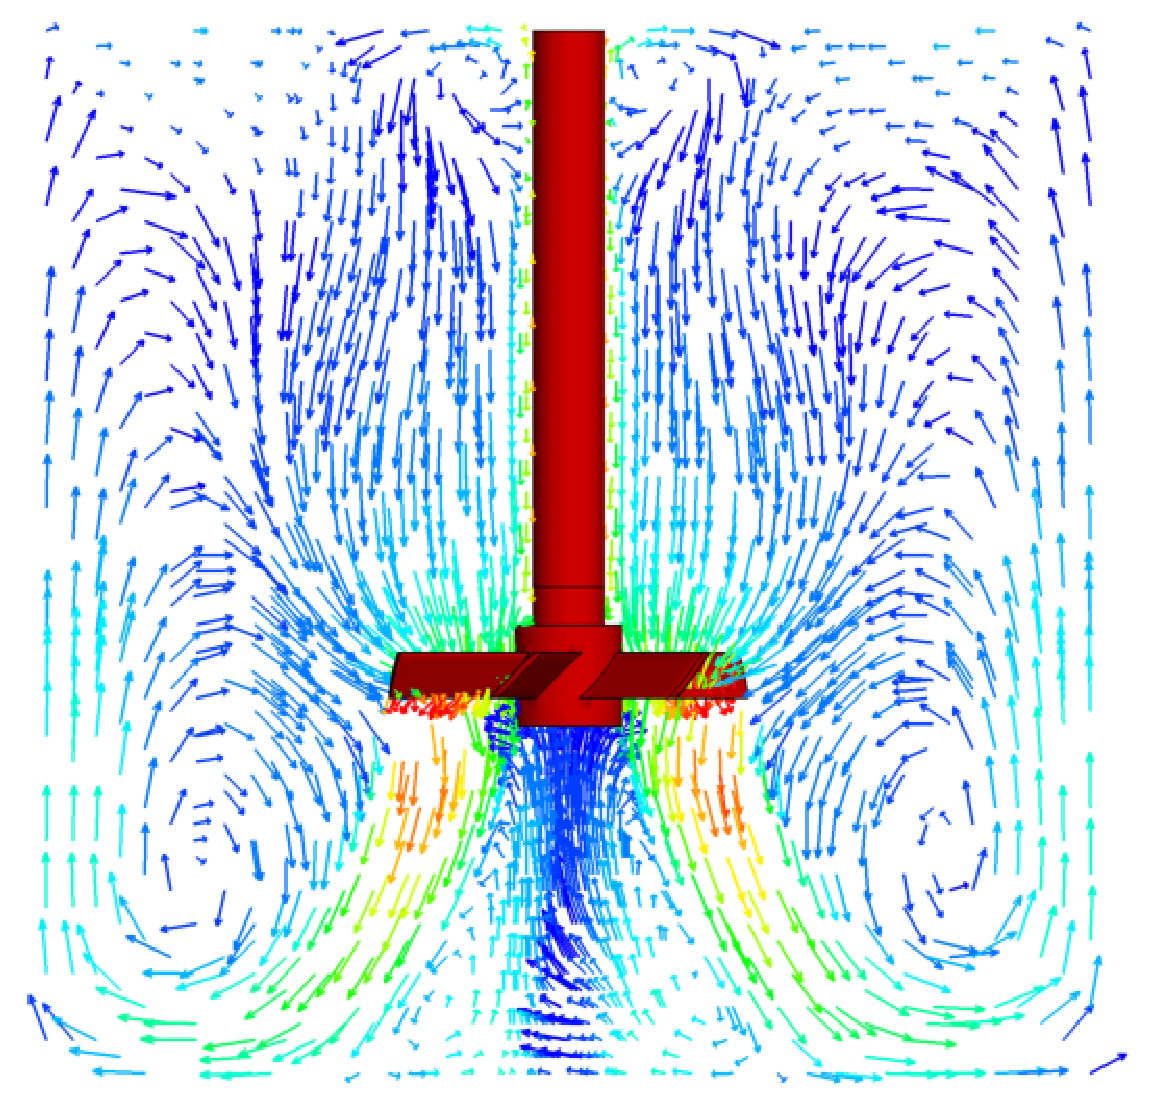
\includegraphics[scale=0.5]{images/vecfield.eps}
\caption{Vektorové pole rychlosti}
\label{fig:vecfield}
\end{center}
\end{figure} 

\vspace{-9mm}

Obr. \ref{fig:count2} zobrazuje kontury objemového zlomku pevné fáze v řezu míchací nádobou pro vybrané korelace odporového koeficientu. Tyto údaje byly získány v času simulace \SI{2}{\second}. Z obrázků je dobře patrné, že přímo pod míchadlem je největší koncentrace pevné fáze vlivem sekundárních cirkulačních smyček. Korelace odporového koeficientu podle Brucata v tomto případě předpovídá významně vyšší rozložení kuliček z PVC pod míchadlem než zbývající modely.

\newpage

\begin{figure}[h!]
  \begin{center}
  \subfloat[Schiller-Naumann]{\label{fig:neu2}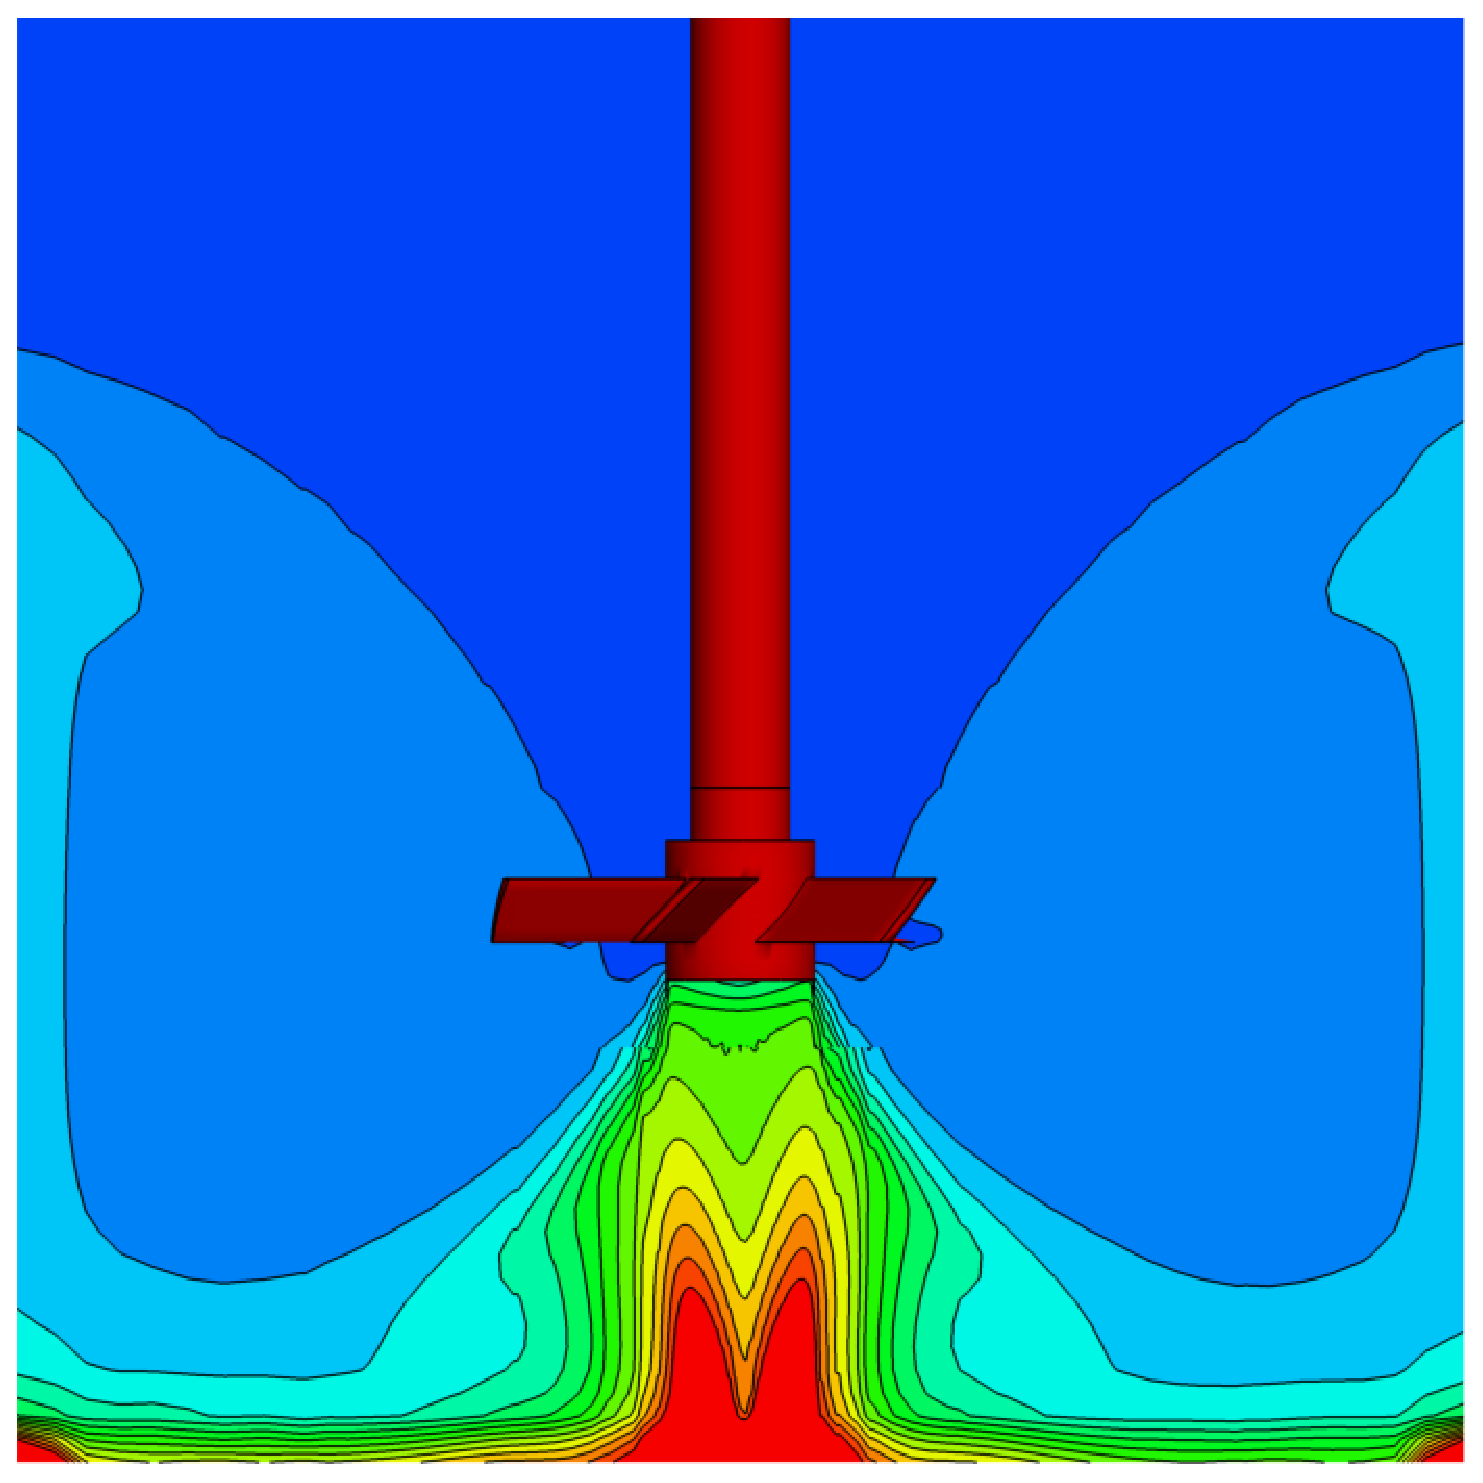
\includegraphics[scale=0.3]{images/volSch-2.eps}}  
  \qquad             
  \subfloat[Pinelli]{\label{fig:pin2}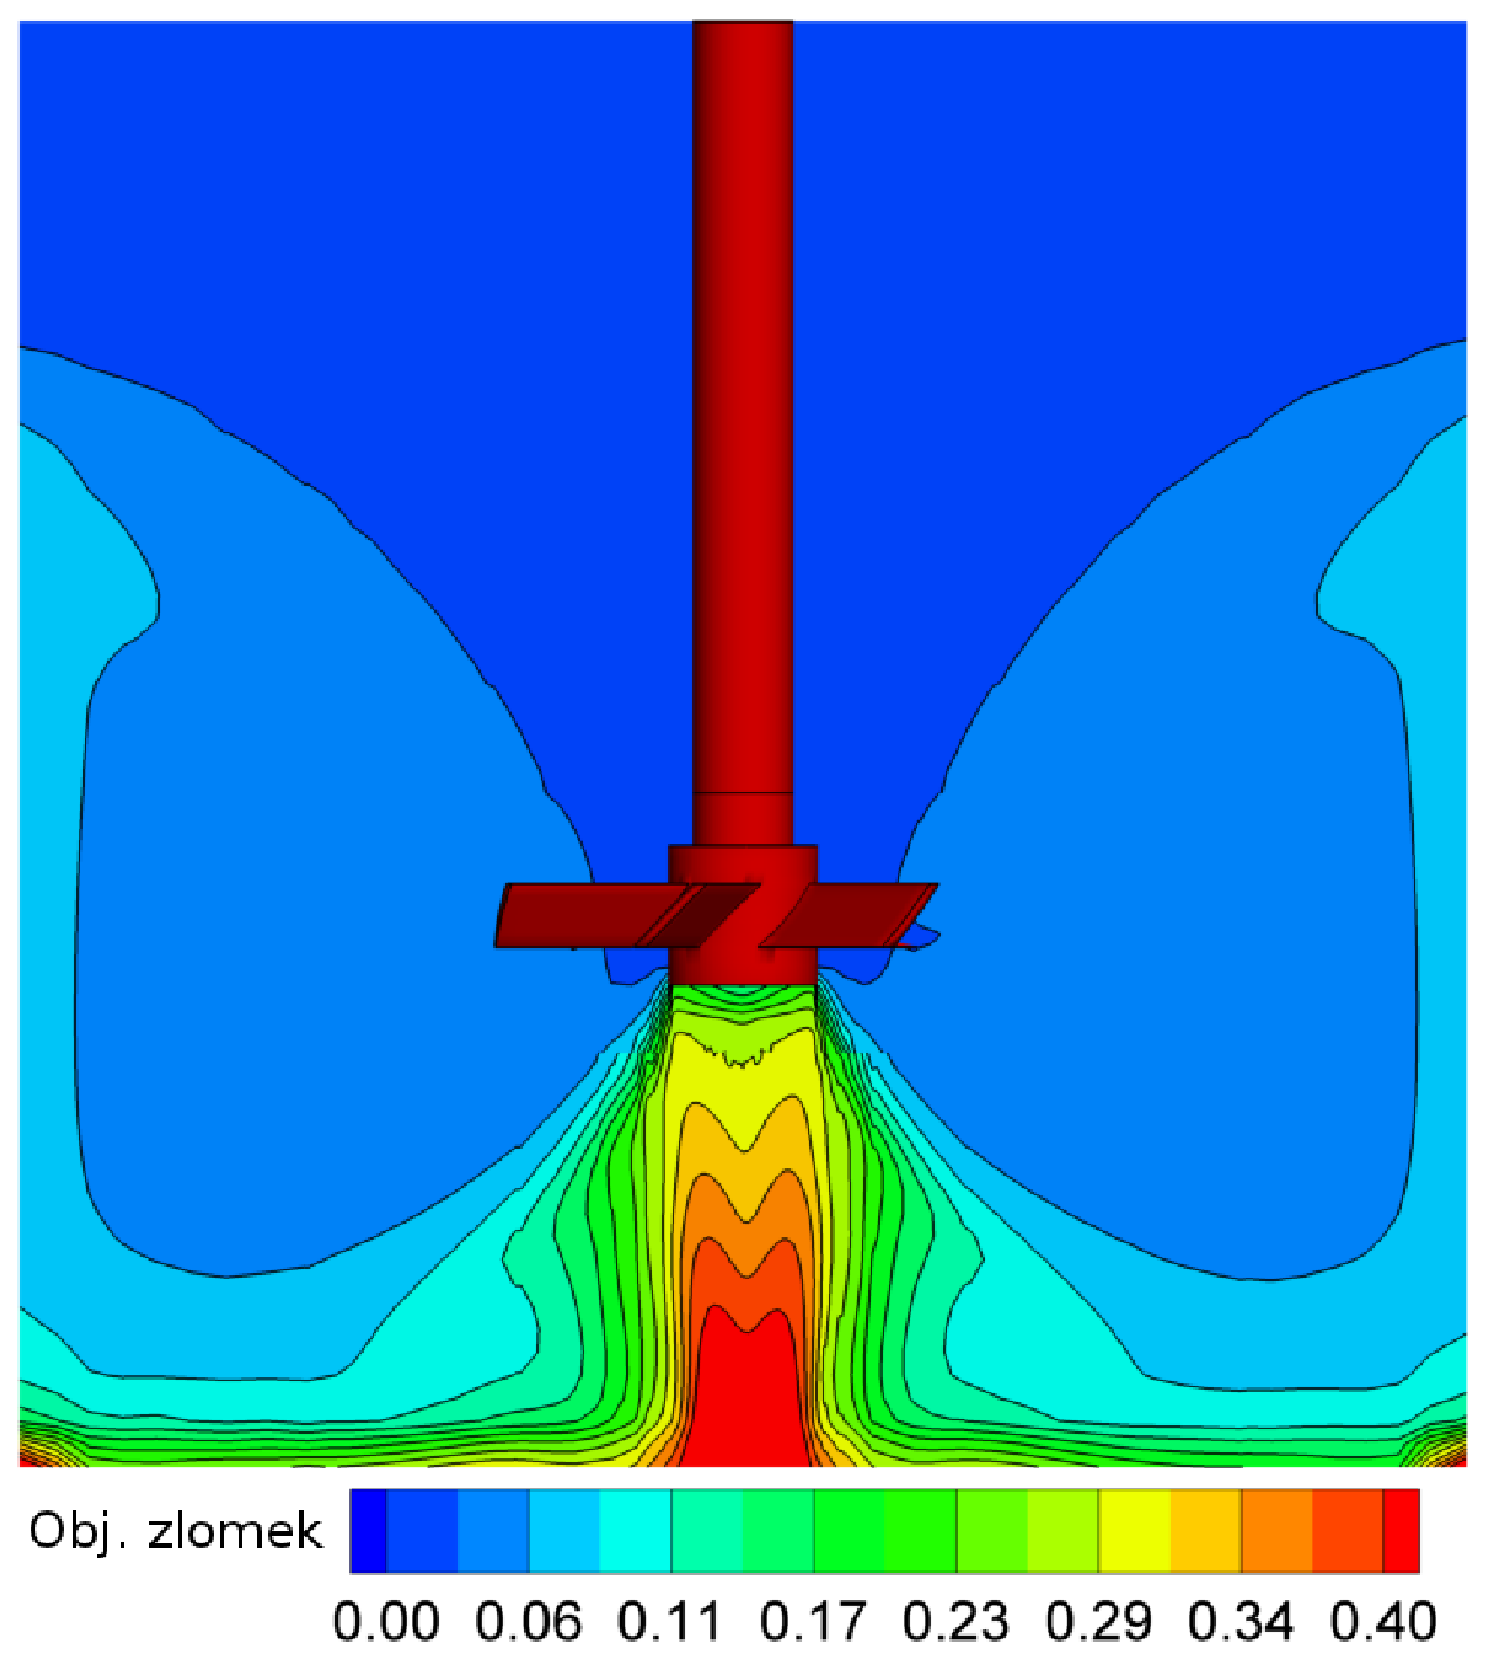
\includegraphics[scale=0.3]{images/volPin-2.eps}}
  \\
  \subfloat[Brucato]{\label{fig:bru2}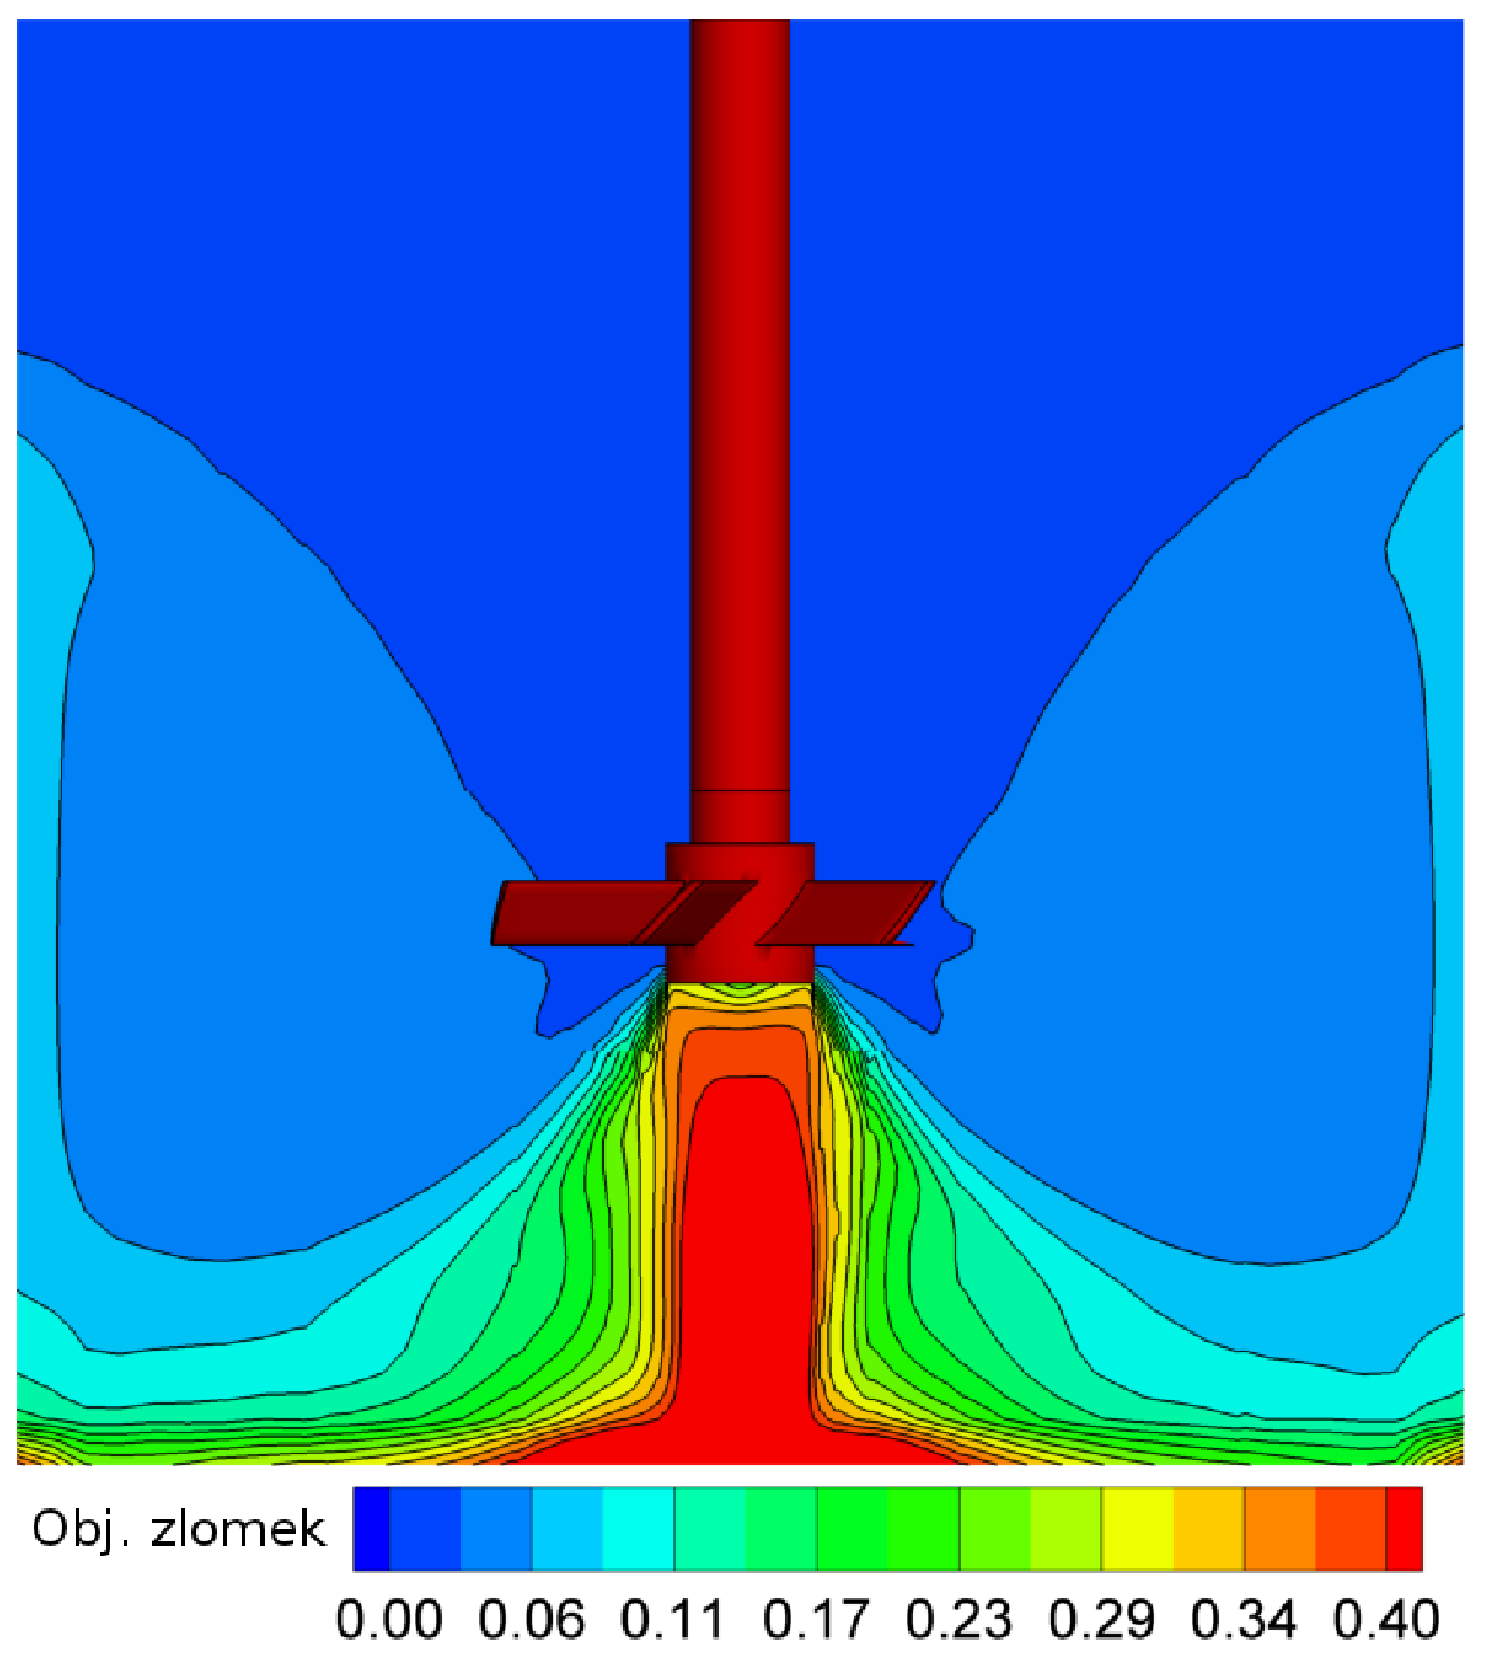
\includegraphics[scale=0.3]{images/volBru-2.eps}}
  \qquad
  \subfloat[Khopkar]{\label{fig:kho2}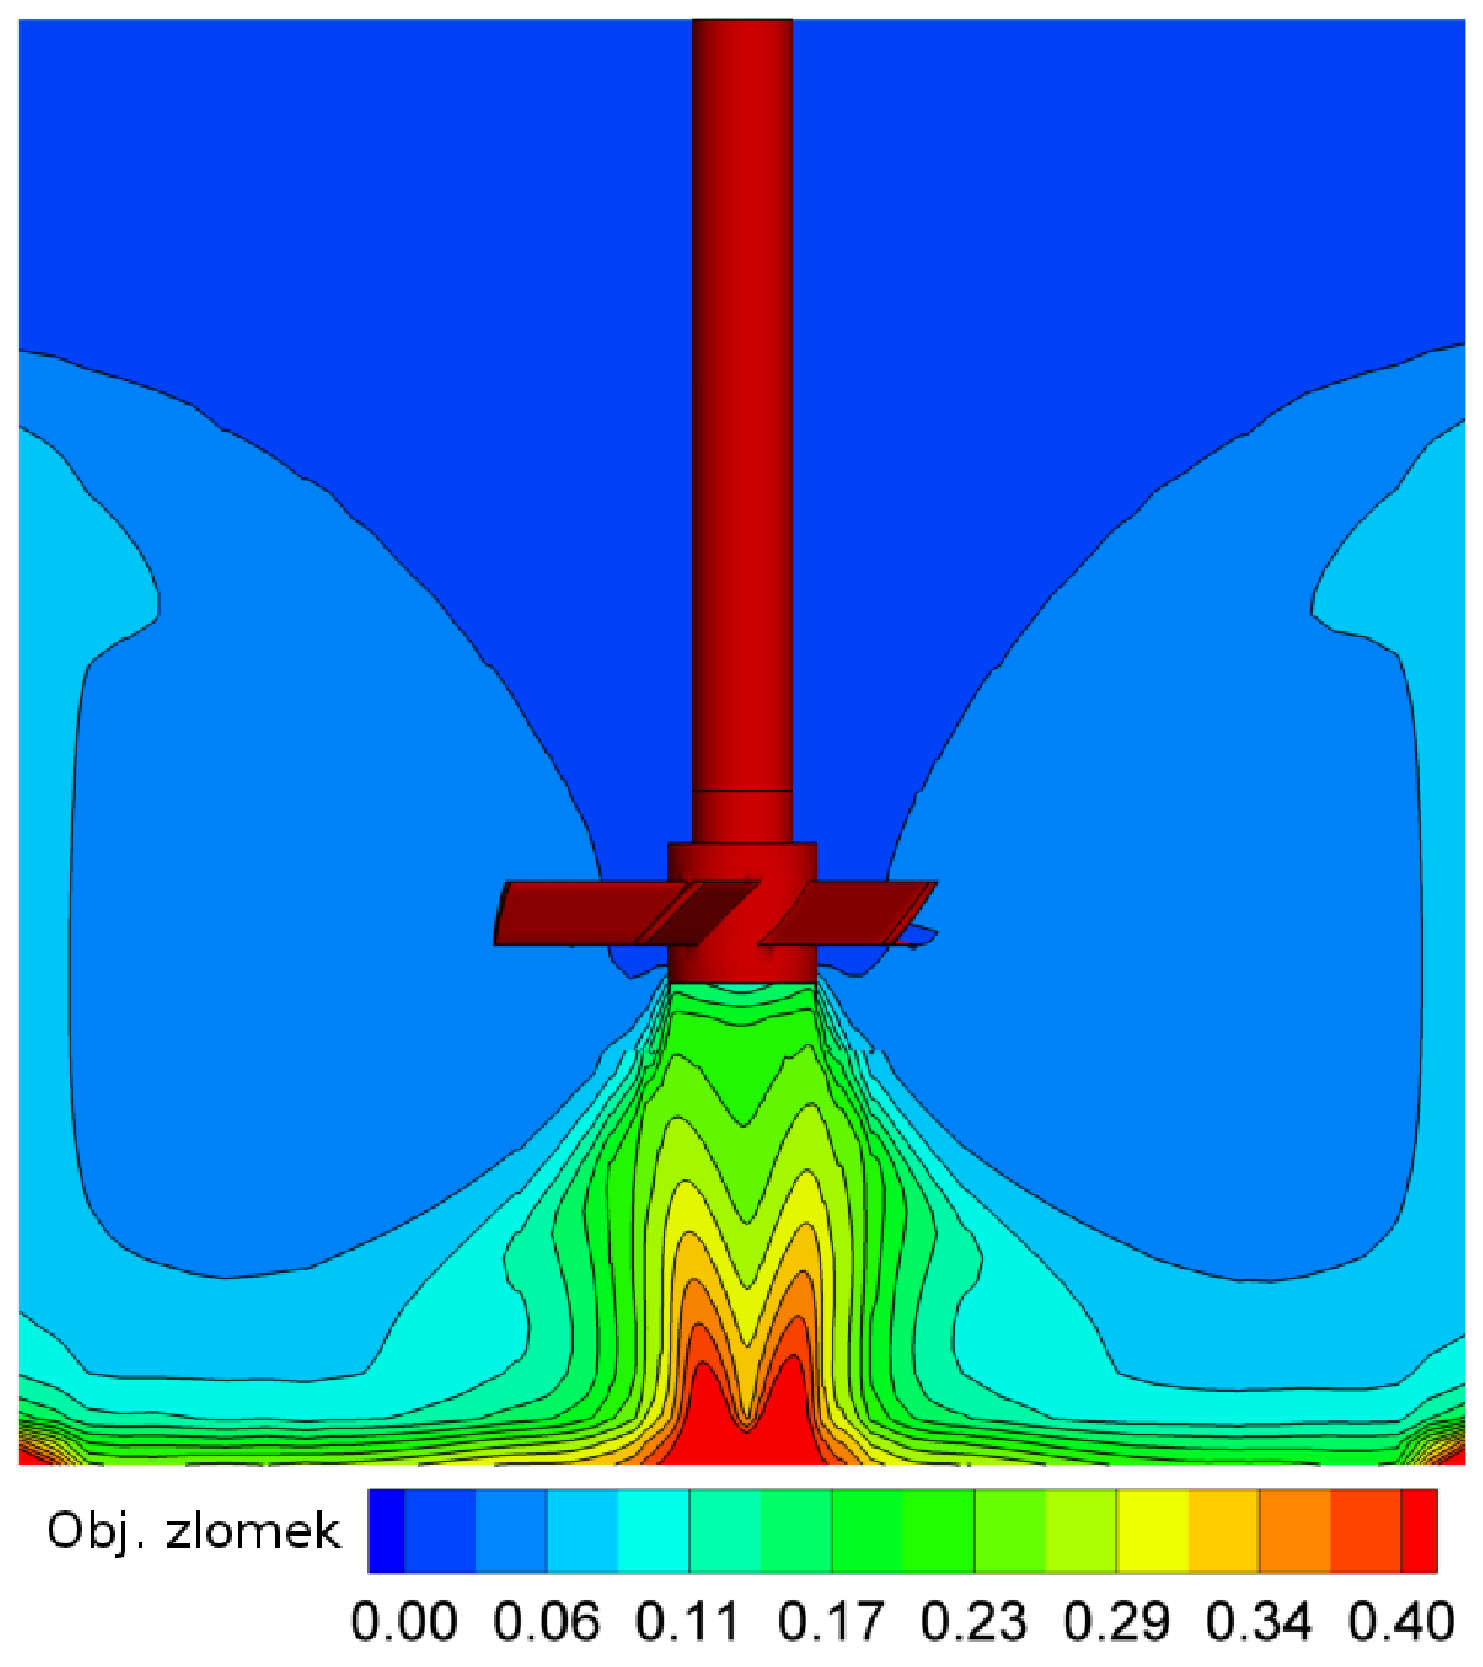
\includegraphics[scale=0.3]{images/volKho-2.eps}}
  \caption{Kocentrace pevné fáze v čase \SI{2}{\second}}
  \label{fig:count2}
  \end{center}
\end{figure}

\vspace{-9mm}

Následují opět obrázky zachycují objemový zlomek pevné fáze v řezu nádobou, avšak v tomto případě pro čas \SI{6}{\second}. Pevná fáze je již poměrně rozptýlena, ale stále se pod míchadlem nacházejí oblasti se zvýšenými koncentracemi.

\newpage

\begin{figure}[h!]
  \begin{center}
  \subfloat[Schiller-Naumann]{\label{fig:neu6}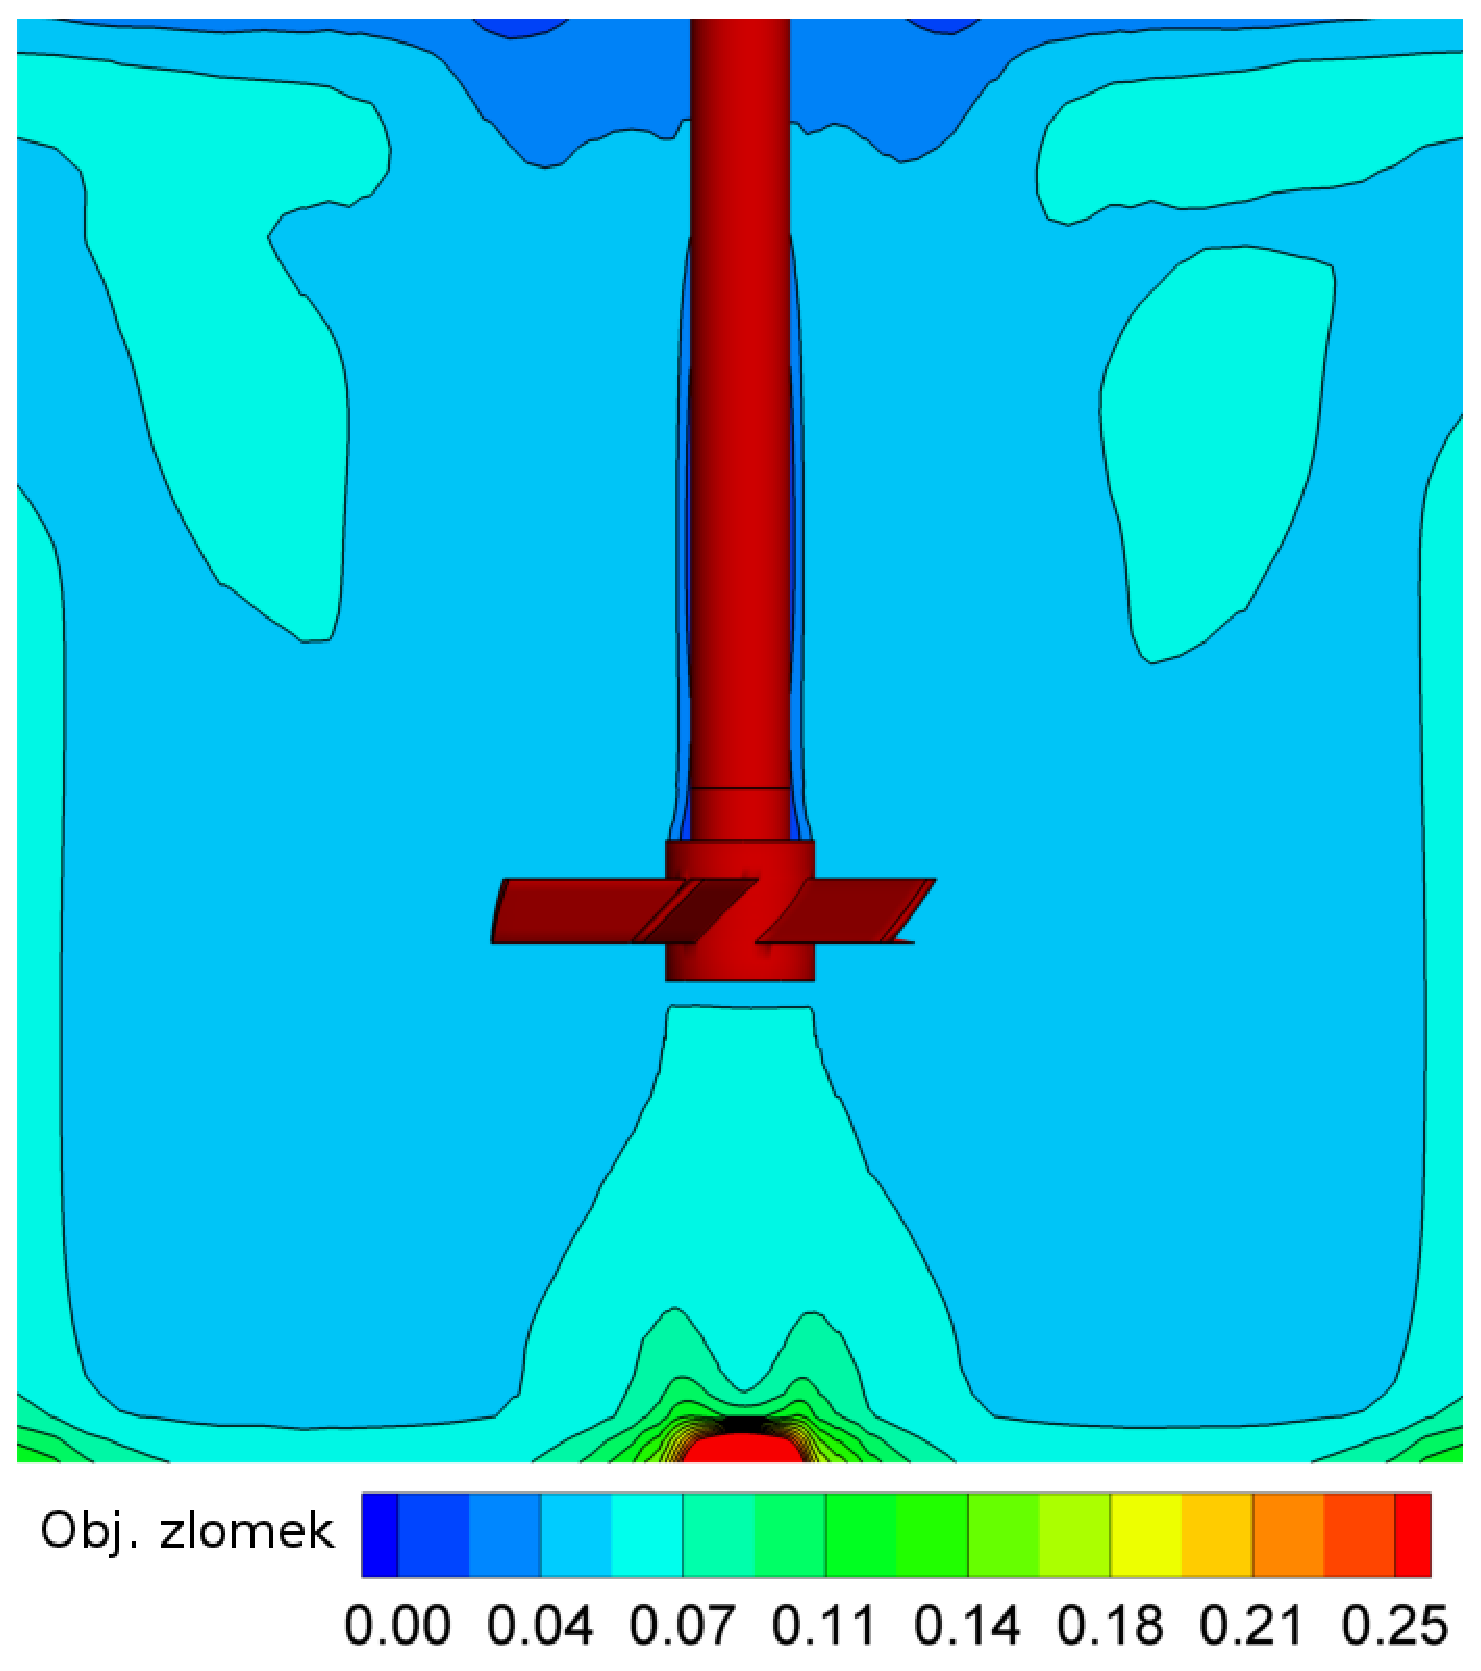
\includegraphics[scale=0.3]{images/volSch-6.eps}}  
  \qquad             
  \subfloat[Pinelli]{\label{fig:pin6}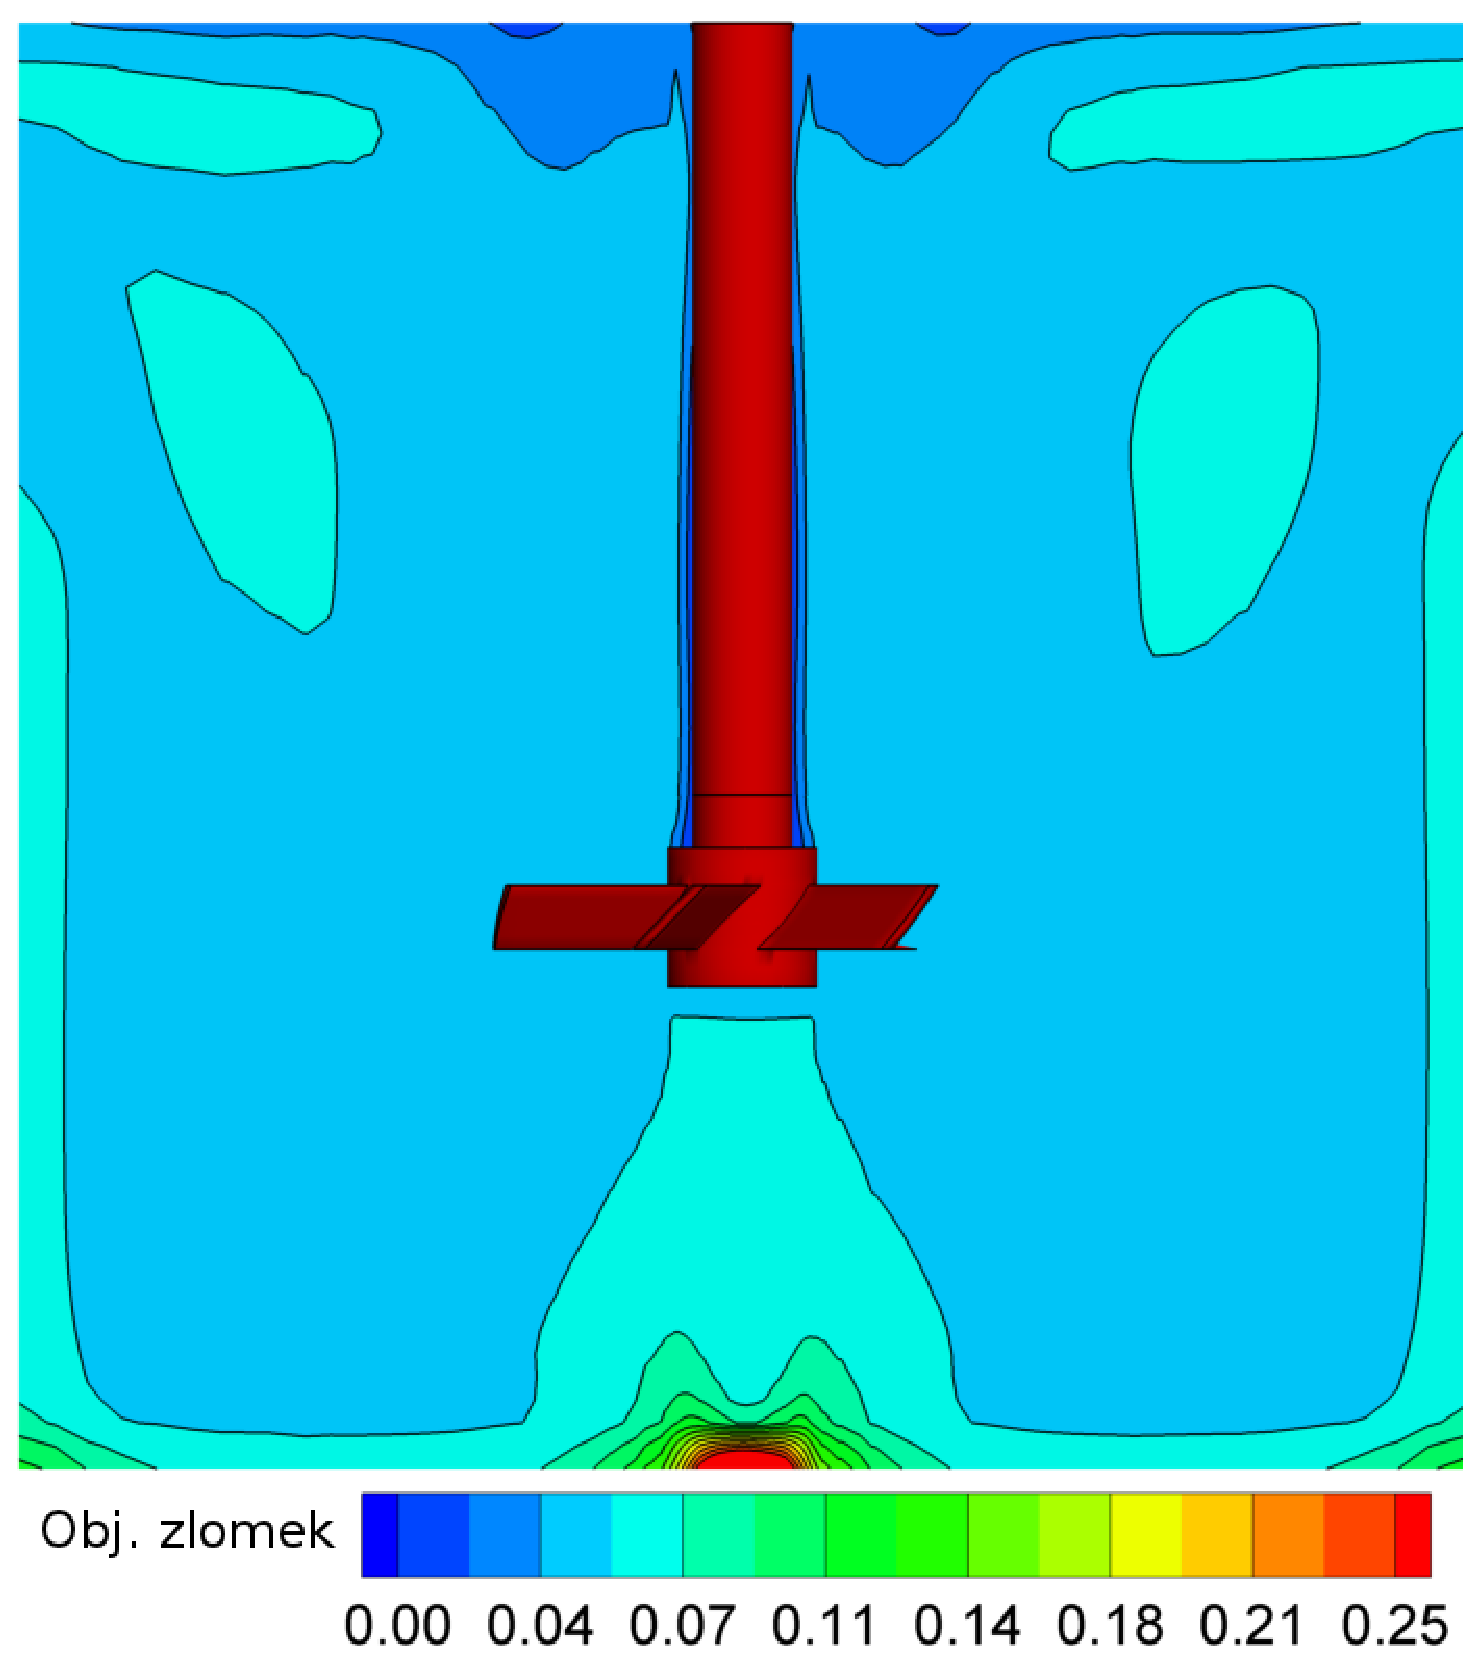
\includegraphics[scale=0.3]{images/volPin-6.eps}}
  \\
  \subfloat[Brucato]{\label{fig:bru6}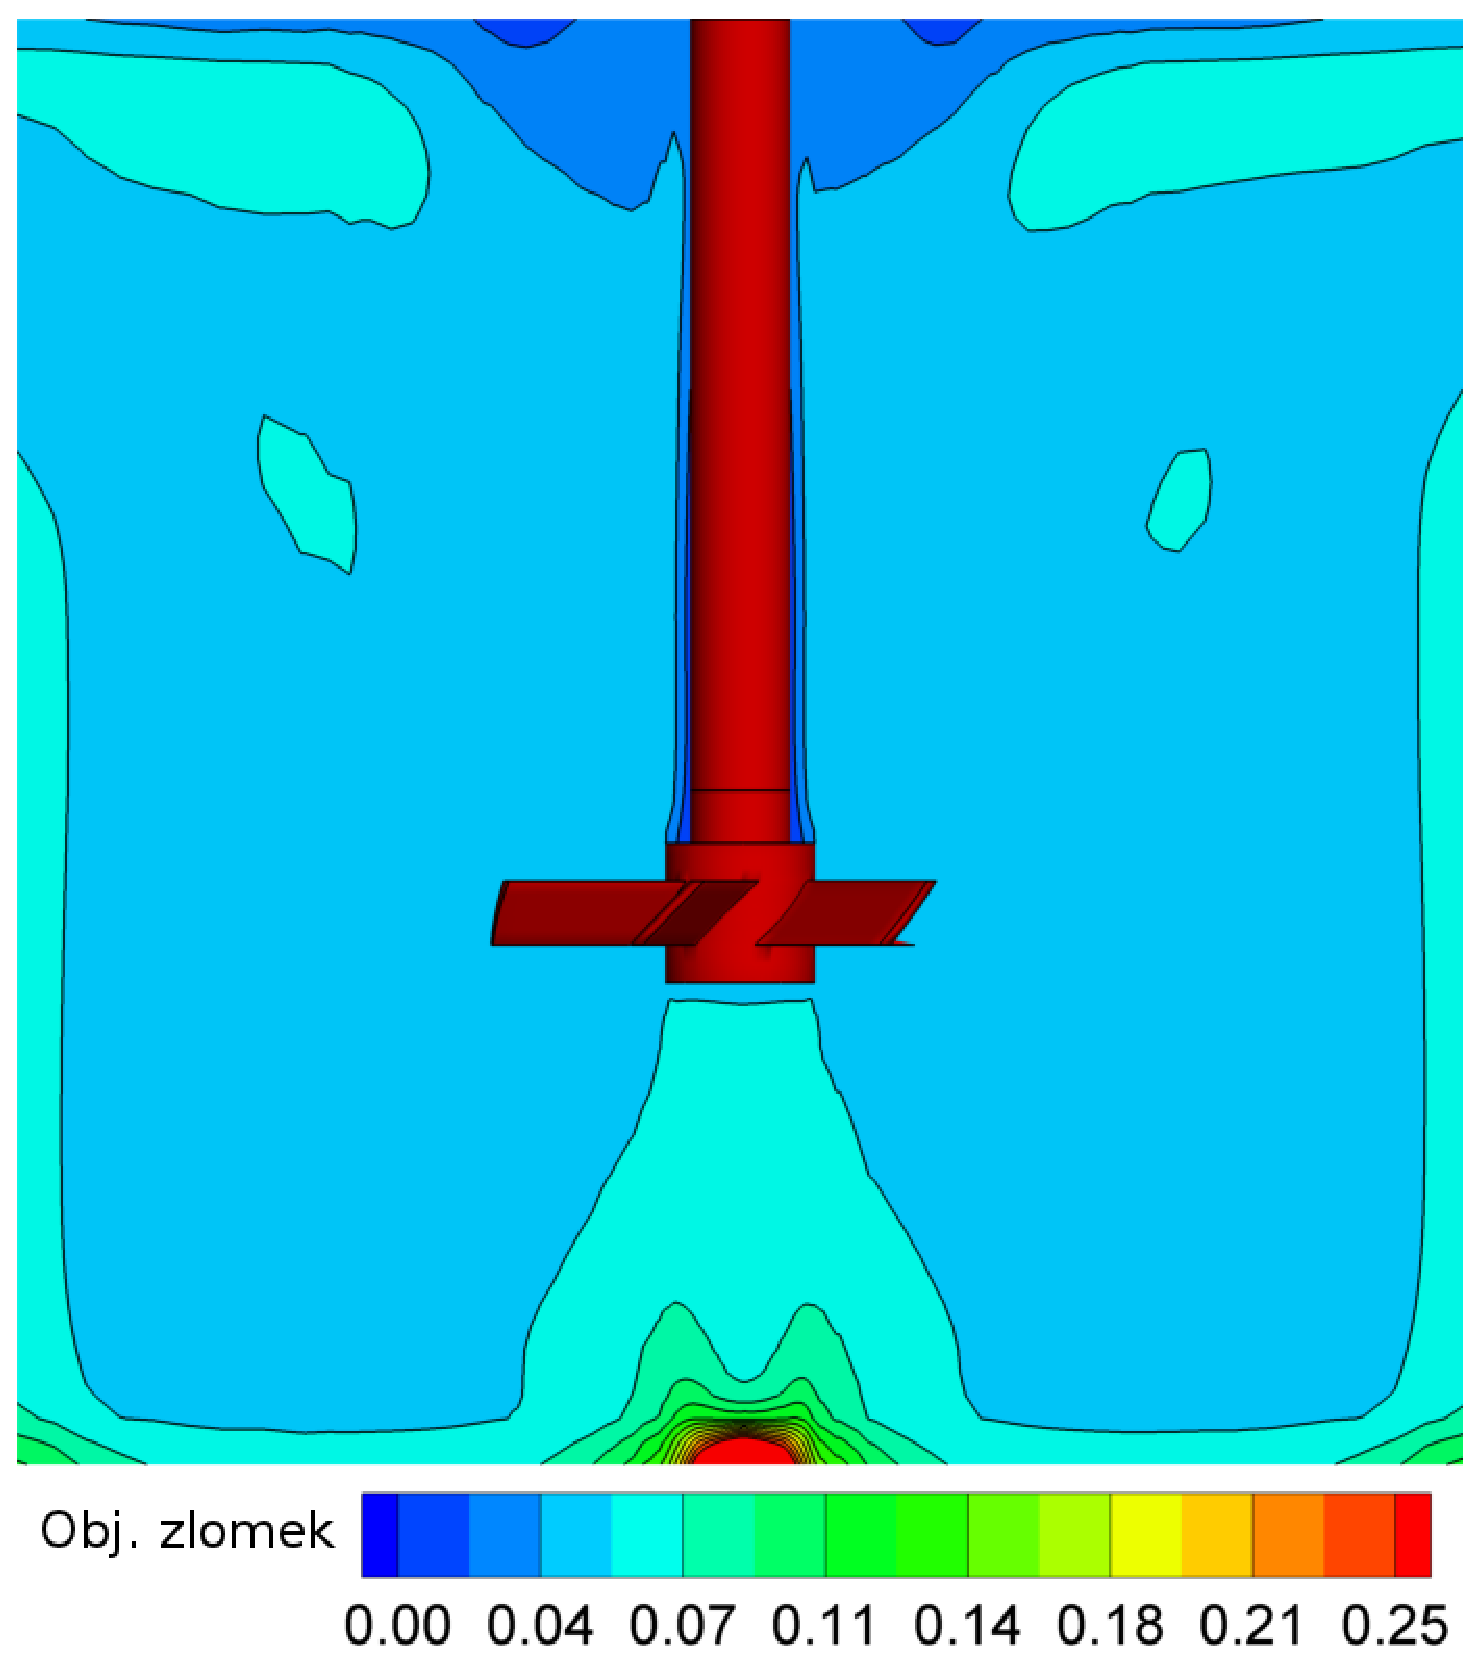
\includegraphics[scale=0.3]{images/volBru-6.eps}}
  \qquad
  \subfloat[Khopkar]{\label{fig:kho6}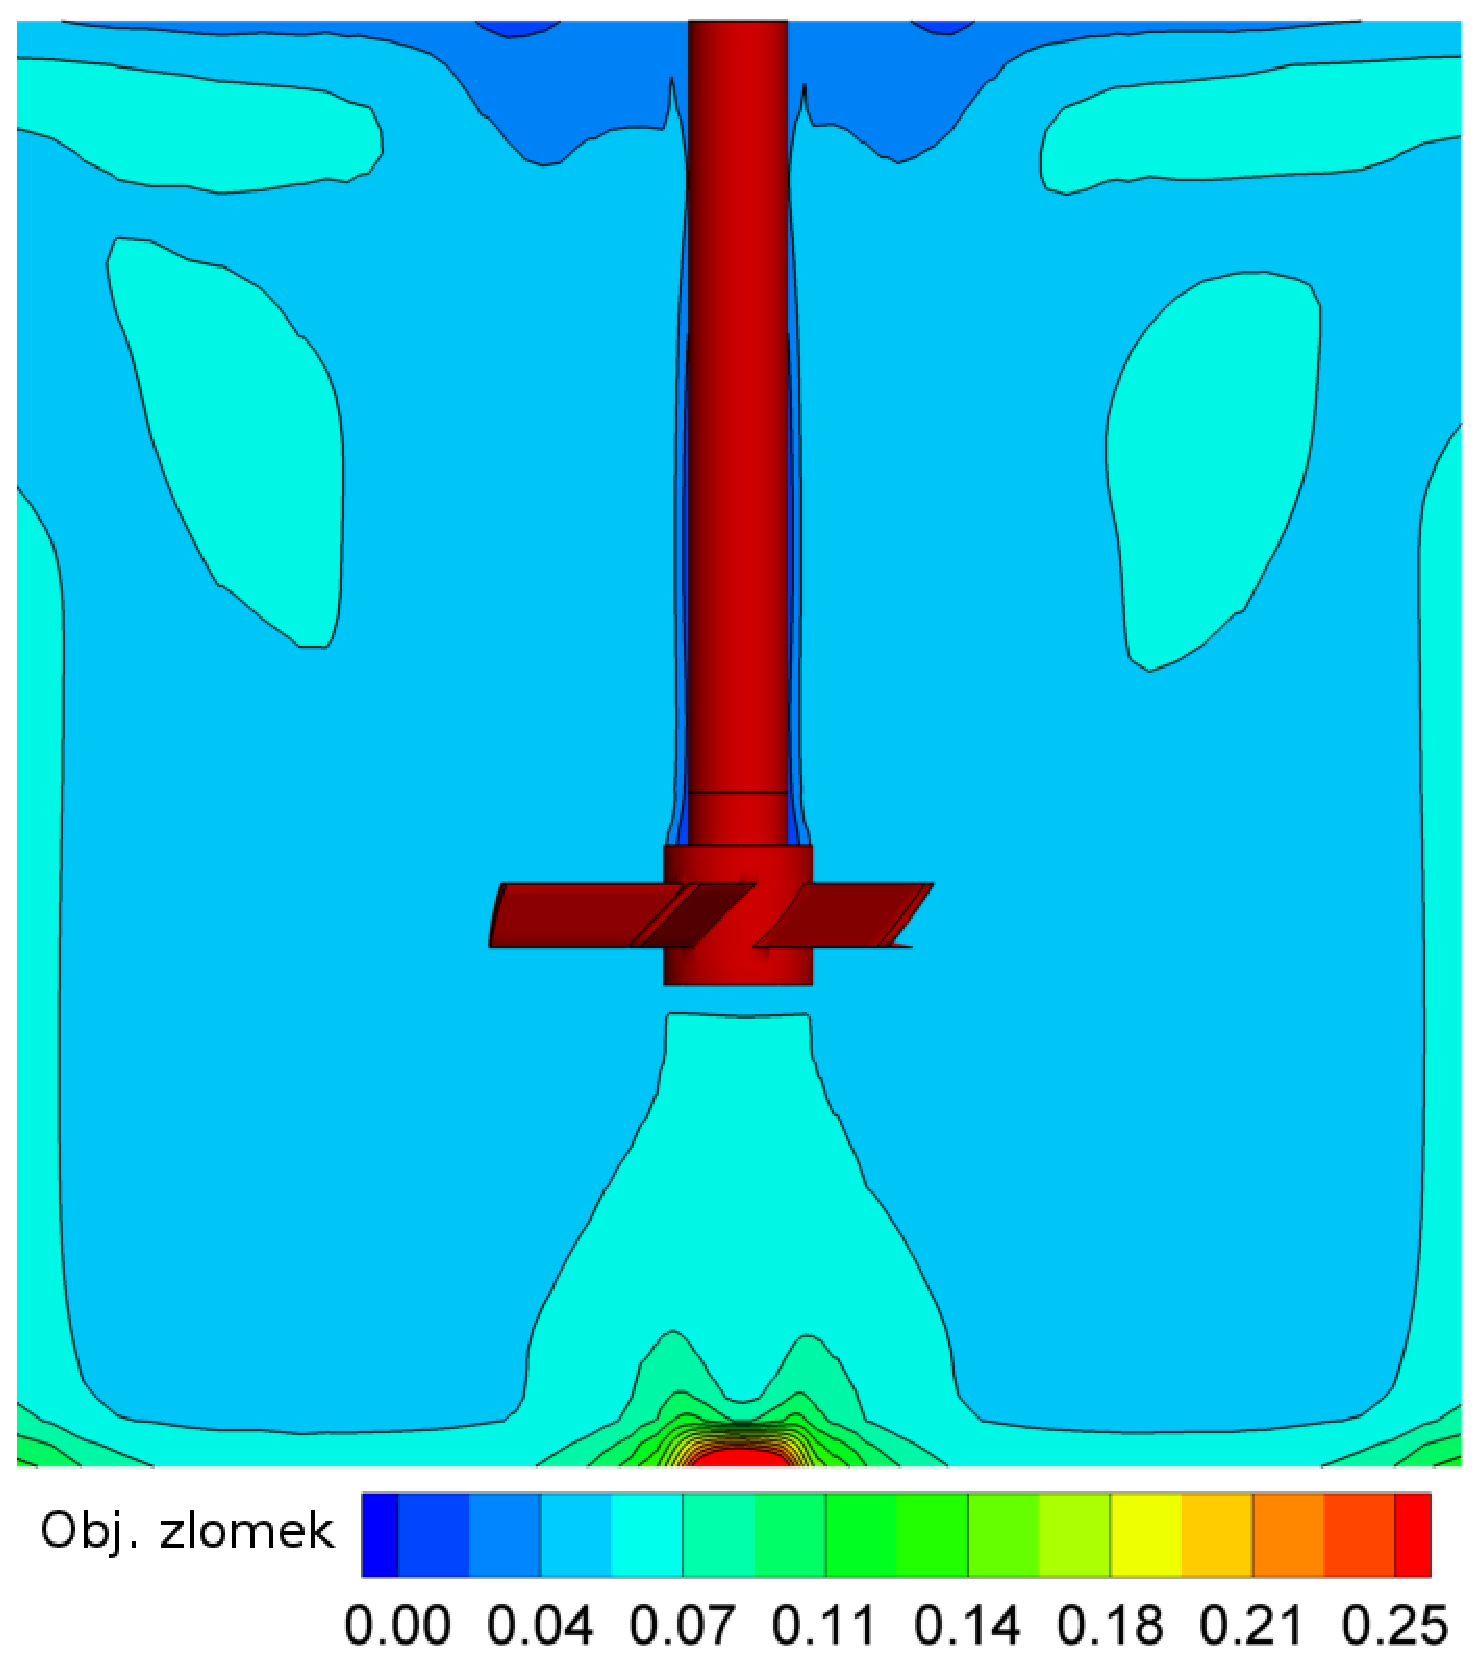
\includegraphics[scale=0.3]{images/volKho-6.eps}}
  \caption{Kocentrace pevné fáze v čase \SI{6}{\second}}
  \label{fig:count6}
  \end{center}
\end{figure}

\vspace{-9mm}

Následují grafické závislosti odporového koeficientu 

\newpage

\begin{figure}[h!]
\begin{center}
\includegraphics[scale=0.47]{images/Vol-2.eps}
\caption{Vektorové pole rychlosti}
\label{fig:vol2}
\end{center}
\end{figure} 

\vspace{-12mm}

\begin{figure}[h!]
\begin{center}
\includegraphics[scale=0.47]{images/Vol-6.eps}
\caption{Vektorové pole rychlosti}
\label{fig:vol6}
\end{center}
\end{figure} 

\vspace{-9mm}

Následují grafické závislosti odporového koeficientu 

\newpage

\begin{figure}[h!]
\begin{center}
\includegraphics[scale=0.47]{images/CD-2.eps}
\caption{Vektorové pole rychlosti}
\label{fig:cd2}
\end{center}
\end{figure} 

\vspace{-12mm}

\begin{figure}[h!]
\begin{center}
\includegraphics[scale=0.47]{images/CD-6.eps}
\caption{Vektorové pole rychlosti}
\label{fig:cd6}
\end{center}
\end{figure} 

\vspace{-9mm}

Následují grafické závislosti odporového koeficientu 


  \chapter{Závěr}
Následující práce byla zaměřena na posouzení vlivu použitého modelu pro koeficient odporu na výsledky CFD simulace suspendace v~mechanicky míchané nádobě. V~rámci této studie bylo implementováno několik korelací pro koeficient odporu v~turbulentní oblasti proudění pomocí uživatelsky definovaných funkcí. Pomocí techniky CFD bylo simulováno promíchávání pevné fáze o~koncentraci 5\,\%\,obj. ve vsádce polyvinylpyrrolidonu.

Ze získaných výsledků vyplynulo, že daný model pro koeficient odporu ovliňuje distribuci pevné fáze zvláště při vyšších objemových zlomcích dané fáze. Tento fakt dobře ilustruje obr. \ref{fig:vol2}. Model navržený \hyperlink{hyp:cds}{Brucatem} pro Taylorův–Couetteovův tok vykazoval ve všech případech výrazně odlišné chování, a proto ho nelze doporučit pro simulaci suspendaci v~mechanicky míchané nádobě. Zbývající modely projevovaly velmi podobné chování, co se týče výsledných koncentračních profilů. 

Budoucí výzkum se zaměří na stanovení výšky vznosu pevné fáze spolu s~určením doby homogenizace a porovnáním s~dostupnými experimentálními výsledky. CFD simulace bude provedena i pro vyšší objemové zlomky pevné fáze spolu se srovnáním dalších vícefázových modelů (např. \nameref{sec:egm}).  


  \addcontentsline{toc}{chapter}{List of symbols}
\chapter*{List of symbols}

\renewcommand\arraystretch{1.5}
\begin{tabularx}{\textwidth}{@{}p{1.0cm} X r@{}}
$N_{js}$ & just suspended impeller speed & \si{\per\second} \\


\end{tabularx}

\subsubsection*{Greek letters}
\begin{tabularx}{\textwidth}{@{}p{1.0cm} X r@{}}
$N_{js}$ & just suspended impeller speed & \si{\per\second} \\
\end{tabularx}

\subsubsection*{Subscripts}
\begin{tabularx}{\textwidth}{@{}p{1.0cm} X r@{}}
$N_{js}$ & just suspended impeller speed & \si{\per\second} \\
\end{tabularx}

\subsubsection*{Shortcuts}
\begin{tabularx}{\textwidth}{@{}p{1.0cm} X }
CFD & computational fluid dynamics  \\
LDV & laser Doppler velocimetry  \\
\end{tabularx}

	\normalsize{}
	%\setlength{\bibhang}{0pt} odsazen prvního řádku bibliografie
	\begin{thebibliography}{99}
\addcontentsline{toc}{chapter}{Literatura}

\bibitem[Armenante \textit{a kol.}, 1998]{arm98} Armenante, P. M., Nagamine, E. U., Susanto, J., 1998. Determination of correlations to predict the minimum agitation speed for complete solid suspension in agitated vessels. \textit{Can J Chem Eng}, \textbf{76}, 413--419

\bibitem[Baldi \textit{a kol.}, 1978]{bal78} Baldi, G., Conti, R., Alaria, E., 1978. Complete suspension of particles in mechanically agitated vessels. \textit{Chem Eng Sci}, \textbf{33}, 21--25 

\bibitem[Brucato \textit{a kol.}, 1998]{bru98} Brucato, A., Grisafi, F., Montante, G., 1998. Particle drag coefficients in turbulent fluids. \textit{Chem Eng Sci}, \textbf{43}, 3, 3295--3314

\bibitem[Clift \textit{a kol.}, 1978]{cli78} Clift, R., Grace, J. R., Weber, M. E.,  1978.  Bubbles, drops, and particles. \textit{Academic Press}, New York

\bibitem[Derksen, 2003]{derk03} Derksen, J.J., 2003. Numerical Simulation of solid suspension in a stirredtank. \textit{AIChE J}, \textbf{49}, 11, 2700--2714

\bibitem[Gidaspow, 1994]{gid94} Gidaspow, D., 1994. Multiphase flow and fluidization: Continuum and kinematic theory description. \textit{Academic Press}, New York

\bibitem[Hosseini \textit{a kol.}, 2010]{hos10} Hosseini, S., Dineshkumar, P., Ein-Mozaffari, F., Mehrvar, M., 2010. Study of Solid-Liquid Mixing in Agitated Tanks through Computational Fluid Dynamics Modeling \textit{Ind. Eng. Chem. Res.}, \textbf{49}, 4426--4435

\bibitem[Ihme \textit{a kol.}, 1972]{ihme72} Ihme, F., Schmidt-Traub H., Brauer, H., 1972. Theoretische untersuchung \"uber die Umstr\"omung und den Stoff\"ubergang an Kugeln. \textit{Chem Ing Tech}, \textbf{44}, 306

\bibitem[Ishii a Zuber, 1979]{ish79} Ishii, M., Zuber, N., 1979, Drag coefficient and relative velocity in bubbly, droplet or particulate flows. \textit{AIChE J}, \textbf{28}, 843--855 

\bibitem[Kasat \textit{a kol.}, 2008]{kas08} Kasat, G. R., Khopkar, A. R., Ranade, V. V., Pandit, A. B., 2008. CFD Simulation of Liquid-Phase Mixing in Solid-Liquid Stirred Reactor. \textit{Chem Eng Sci}, \textbf{63}, 3877--3885

\bibitem[Khopkar \textit{a kol.}, 2006]{kho06} Khopkar, A. R., Kasat, G. R., Pandit, A. B., Ranade, V. V., 2006. Computational Fluid Dynamics Simulation of Solid Suspension in Stirred Slurry Seactor. \textit{Ind Eng Chem Res} \textbf{45}, 4416--4428.

\bibitem[Kresta a Wood, 1991]{kre91} Kresta, S. M., Wood, P. E., 1991. Prediction of three-dimensional turbulent flow in stirred tanks. \textit{AIChE J}, \textbf{37}, 448--460 

\bibitem[Ljungqvist a Rasmuson, 2001]{lju01} Ljungqvist, M., Rasmuson, A., 2001. Numerical simulation of the two-phase flow in an axially stirred reactor. \textit{Trans AIChE}, \textbf{79}, Part A, 533--546

\bibitem[Micale \textit{a kol.}, 2003]{mic04} Micale, G., Grisafi, F., Rizzuti, L., Brucato, A., 2004. CFD simulation of particle suspension height in stirred vessels. \textit{Chem Eng Res Des}, \textbf{82}, 1204--1213

\bibitem[Micheletti \textit{a kol.}, 2003]{miche03} Micheletti, L., Nikiforaki, L., Lee, K. C., Yianeeskis, M., 2003. Integral and Local Concentration Characteristics of Moderate to Dense Solid-Liquid Suspensions. \textit{11$^{th}$ European Conference on Mixing}, Bamberg, Germany

\bibitem[Montante a Bakker, 2004]{mon04} Montante, G., Bakker, A., 2004, Solid-Liquid Multiphase Flow Validation in Tall Stirred Vessels with Multiple Impeller Systems \textit{Technical Notes}, \textbf{TN253}, Fluent Inc.

\bibitem[např.\ Nienow, 1968]{nie68} Nienow, A. W., 1968. Suspension of solid particles in turbine agitated baffled vessels. \textit{Chem Eng Sci}, \textbf{23}, 1453--1459 

\bibitem[Ochieng a Onyango, 2008]{ochi08} Ochieng, A., Onyango, M. S., 2008. Drag models, solids concentration and velocity distribution in a stirred tank. \textit{Pow Tech}, \textbf{181}, 1--8

\bibitem[Oshinowo a Bakker, 2002]{oshi02} Oshinowo, L. M., Bakker, A., 2002. CFD modeling of solids suspensions in stirred tanks. \textit{Symposium on Computational Modeling of Metals, Minerals and Materials}, February 17-21, Seattle, Washington 

\bibitem[Pinellim \textit{a kol.}, 2001]{pin01} Pinelli, D., Nocentini, M., Magelli, F., 2001. Solids distribution in stirred slurry reactors: in influence of some mixer configurations and limits to the applicability of a simple model for predictions.
\textit{Chem Eng Comm}, \textbf{188}, 91--107

\bibitem[Schiller a Naumann, 1935]{schi32} Schiller, L., Naumann, Z., 1935. A drag coefficient correlation. \textit{Z. Ver. Deutsch. Ing.}, \textbf{77}, 318--320

\bibitem[Syamlalem a O'Brienem, 1993]{syam93} Syamlal, M., O'Brien, T. J., 1993. MFIX Documentation: Theory Guide. \textit{National Technical Information Service}, \textbf{1}, Springfield, Virginia 

\bibitem[Tamburini \textit{a kol.}, 2009]{tamb09} Tamburini, A., Cipollina, A., Micale, G., Ciofalo, M., Brucato, A., 2009. Dense solid–liquid off-bottom suspension dynamics: Simulation and experiment. \textit{Chem Eng Res Des}, \textbf{87}, 587--597

\bibitem[Yamazaki \textit{a kol.}, 2008]{yama08} Yamazaki, H., Tojo, K., Miyanami, K., 1986. Concentration profiles of solids suspended in a stirred tank. \textit{Pow Tech}, \textbf{48}, 205--216

\bibitem[Zwietering, 1957]{zwi58} Zwietering, T. N., 1958. Suspending of solid particles in liquid by agitators. \textit{Chem Eng Sci}, \textbf{8}, 244--253 

\end{thebibliography}

  \chapter*{Příloha}
\label{sec:priloha}
\addcontentsline{toc}{chapter}{Příloha}
Zde jsou uvedeny vytvořené zdrojové kódy uživatelsky definovaných funkcí pro dané modely koeficientu odporu. Online repositář je možné nalézt na adrese \href{http://code.google.com/p/mixing-udfs/source/browse/\#hg\%2FDragCoefModels}{http://code.google.com/p/mixing-udfs/source/browse/\#hg\%2FDragCoefModels}. 



\lstinputlisting{Models.c}

\lstinputlisting{SchillerNauman.h}
  
\end{document}
